\section{Systematic Uncertainties}
\label{sec:systematics}

\subsection{Background}
The systematic uncertainty on the estimated background differs depending on the final selection
 as listed in Table \ref{tab:background}. The relative systematic uncertainty is estimated using the prescription
described in Section \ref{subsec:abcd}. It is evaluated to be 32\% and 46\%
for {\it low} and {\it high} $L_{xy}$ selections with 1.60 and 1.14 predicted background candidates respectively. 
The 7 background predictions from which the systematic uncertainty is derived are listed in Table \ref{tab:sigbkg}.

\begin{table}[htbp]
\centering
\caption{Predicted background level for the final selections obtained with 7 combinations using the
method of independent selections. \label{tab:sigbkg}}

\begin{tabular}{lcc}

\hline
Selection & {\it low} $L_{xy} $& {\it high} $L_{xy}$ \\
\hline
$BCD/A^2$ & 1.60 & 1.14 \\
$FG/B$ & 1.21 & 1.00 \\
$EG/C$ & 1.92 & 0.84 \\
$DG/A$ & 1.76 & 1.25 \\
$BE/A$ & 1.72 & 0.77 \\
$CF/A$ & 1.08 & 0.92 \\
$EF/D$ & 1.16 & 0.62 \\
\hline

\end{tabular}
\end{table} 


\subsection{Luminosity}
For the running period corresponding to this analysis, CMS estimates the relative uncertainty on the luminosity to be 4.4\% \cite{CMS-PAS-LUM-12-001}.

\subsection{Effect of Pile-Up}
The likelihood of a given number of pile-up events occurring in the data can be calculated from the distribution
 of the instantaneous luminosity during the 2012 run. The number of true pile-up events in the Monte Carlo
 simulation is also known. The simulation can therefore be re-weighted to match the data. 

The systematic uncertainty in this procedure is estimated by adjusting the re-weighting, so as to account
 for uncertainties related to pile-up modeling. 
The effect of a $\pm$5\% variation in the number of interactions is estimated and gives rise 
to a relative systematic uncertainty in the signal reconstruction efficiency 
of less than 2\% for all mass and lifetime points considered. The signal reconstruction efficiency as
a function of number of primary pile-up vertices is shown in Figure \ref{fig:effPU}. No significant
decrease in efficiency is observed as the number of primary pile-up vertices increases.

\begin{figure}[htbp]
\centering
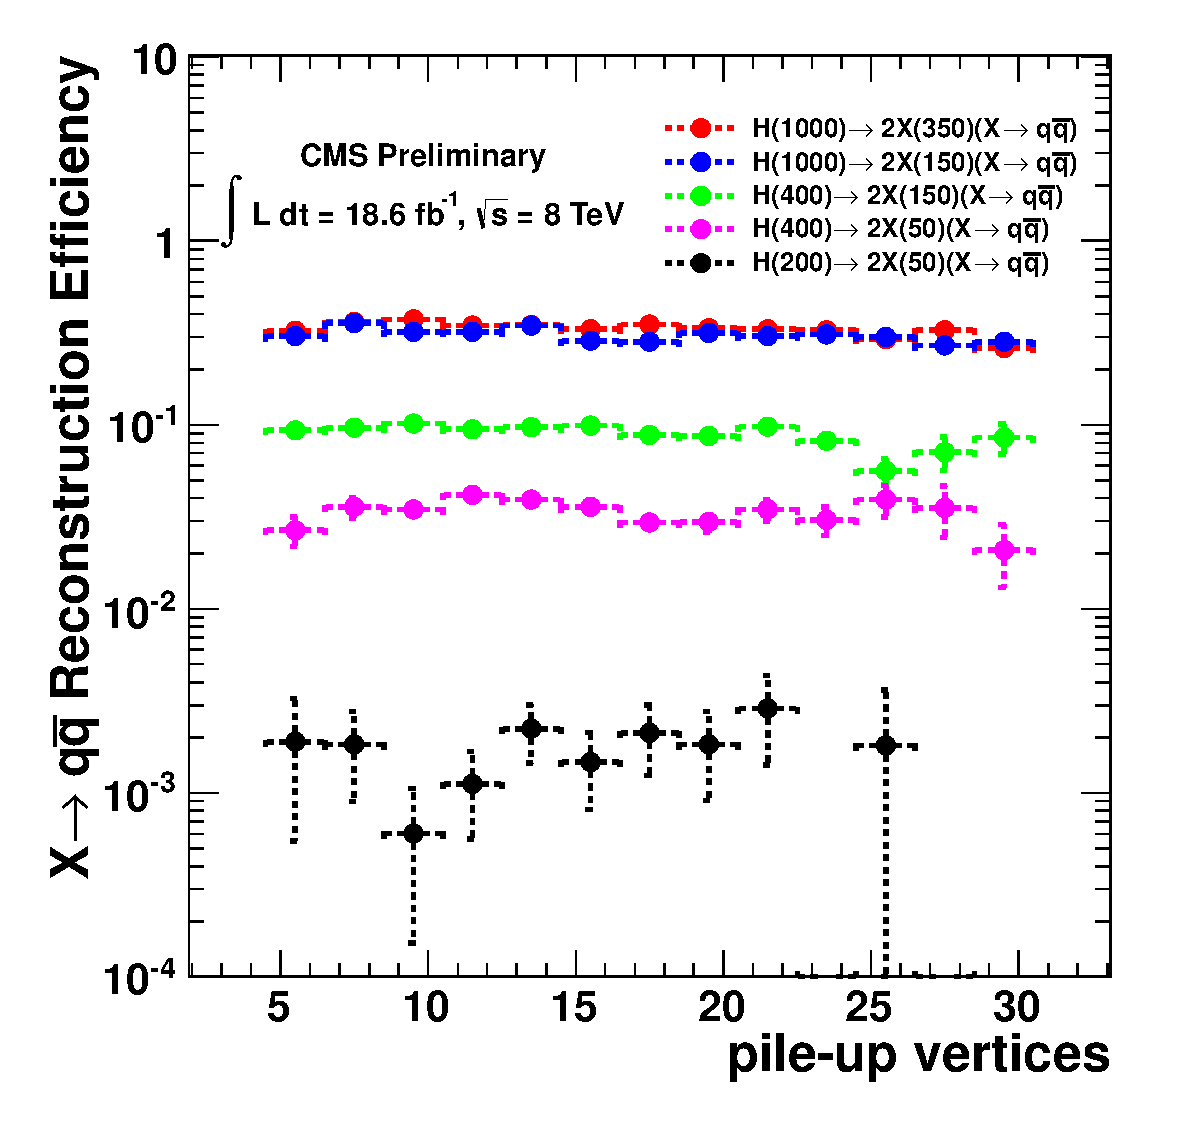
\includegraphics[width=0.49\textwidth]{plots/signal/effPU.pdf}
\caption{Reconstruction efficiency as a function of number of pile-up vertices for selected
signal models.\label{fig:effPU}}
\end{figure}

\subsection{Primary vertex selection}
\label{subsec:pv}
The relevant impact parameters and decay lengths are computed 
with respect to the primary vertex which has the highest
squared transverse momentum sum of the tracks. If a dijet candidate does not originate from this vertex the impact
parameters would be computed incorrectly. The size of the luminous region, where the primary vertices lie,
 is $\sim$5\cm in the longitudinal direction and $\sim$15$\mu m$ in both transverse directions. 
Therefore the effect of an incorrect primary vertex assignment significantly increases the 3-D impact parameters,
 while for
the transverse impact parameters the effect is small as the size of the luminous region is smaller than the 
primary vertex resolution (20$\mu m$).
In the displaced dijet selection criteria the 3-D impact parameters are used to compute 
the number of jet prompt tracks, while all other criteria employ
only the transverse impact parameters. 
 We study the background level and signal reconstruction efficiency where all
 the relevant impact parameters and
decay lengths are computed with respect to the second, instead of the first, primary vertex. In this scenario 
the selection of an incorrect primary vertex is greatly enhanced. The predicted and
observed background level are detailed in Table \ref{tab:wrongvtx}.

\begin{table}[htbp]
\caption{Predicted and observed background for the optimised selections for first and second highest squared transverse momentum sum primary vertex in the event. Uncertainties on the background level include both statistical
and systematic uncertainties. \label{tab:wrongvtx}}
\begin{tabular}{lcccc}
\hline
selection & low $L_{xy}$ (1$^{st}$ PV) & high $L_{xy}$ (1$^{st}$ PV) & low $L_{xy}$ (2$^{nd}$ PV) & high $L_{xy}$ (2$^{nd}$ PV)\\
\hline
predicted bkg. & $1.60\pm0.57$ & $1.14\pm0.54$ & $1.67\pm0.75$ & $1.17\pm0.66$ \\
observed bkg. & 2 & 1 & 2 & 1 \\ 
\hline
\end{tabular}
\end{table}

The predicted background level minimally increases if a wrong primary vertex is used, while the increase is small
with respect to the background level uncertainty. The signal reconstruction efficiency 
does not significantly change whether the first or second leading primary vertex is used.

\subsection{Displaced Tracking Efficiency}

The signal reconstruction efficiency is obtained assuming the tracking efficiency is correctly 
accounted for in the MC simulation. In order to validate this assumption we study
the relative tracking efficiency as functions of displacement and pile-up using
$\Kshort \to \pi^+\pi^-$ decays in data and simulation.
The $\Kshort \to \pi^+\pi^-$ decay mode, with the \Kshort proper decay length of $2.68 \cm$
 \cite{Beringer:1900zz}, provides an abundant source of tracks originating
at displaced locations. 
The tracking efficiency for \Kshort pions can be used to check the displaced jet tracking efficiency, 
as the jet tracks consist mostly of low momentum light hadrons. 

\subsubsection{Pion displaced tracking efficiency}
\label{subsubsec:pitrkeff}

Data and simulation events are selected with the HLT\_HT300 trigger, thus providing
a source of \Kshort decays in a jet environment. The pile-up distribution in simulation is re-weighted
to match the corresponding distribution in data. 
To obtain a clean sample of \Kshort, pairs of {\it high-purity} tracks with $p_T>1$\GeV are combined
 into a secondary 
vertex with the following criteria:
\begin{itemize}
 \item secondary vertex $\chi^2/$degree of freedom $<$ 7
 \item decay length significance of the secondary vertex $>$ 5
 \item significance of the three-dimensional impact parameters for both pion tracks $>$ 3
 \item significance of the three-dimensional impact parameter of the \Kshort candidate $<$ 3 
\end{itemize}
where the decay lengths and impact parameters are computed with respect to the leading primary vertex
in the event.
The secondary vertex invariant mass distribution is shown in Figure \ref{fig:ksmass}. 
In Figure \ref{fig:ksmass}, as well as all other figures
presented in this section, in order to reduce the effect of statistical fluctuations, 
the data/simulation ratio histograms are shown with neighbouring bins merged until the
relative statistical uncertainty does not exceed 2\%. 

\begin{figure}[htbp]
\centering
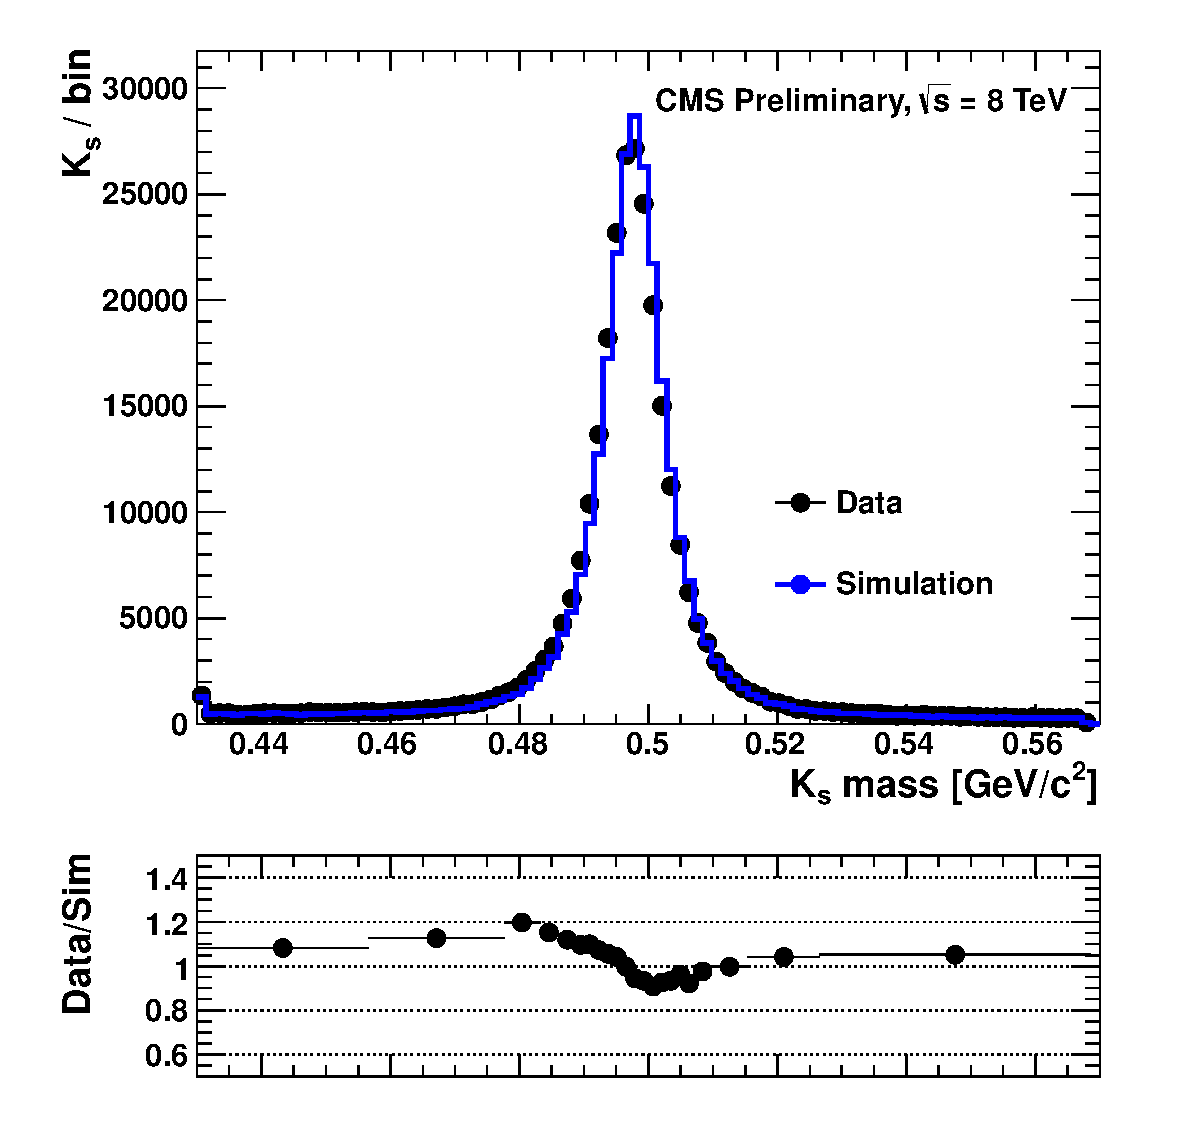
\includegraphics[width=0.49\textwidth]{plots/kshort/ksmass.pdf}
\caption{Invariant mass distribution of the \Kshort candidates in data and simulation. \label{fig:ksmass}}
\end{figure} 


The mean lifetime of the \Kshort is known with better than 0.1\% precision, however the \Kshort
production rate as well as its kinematic distributions are not perfectly reproduced 
by \PYTHIA \cite{Khachatryan:2011tm}.
In order to remove a potential bias arising from the generator level discrepancies, 
we select the \Kshort candidates with transverse decay length $L_{xy}<2\cm$ where tracking efficiency
is high and well simulated. We then compare $p_T$ and $\eta$ distributions for these candidates and obtain
weights, binned in $p_T$ and $\eta$, as well as an overall scale factor which are further
 applied for all \Kshort candidates. 

\begin{figure}[htbp]
\centering
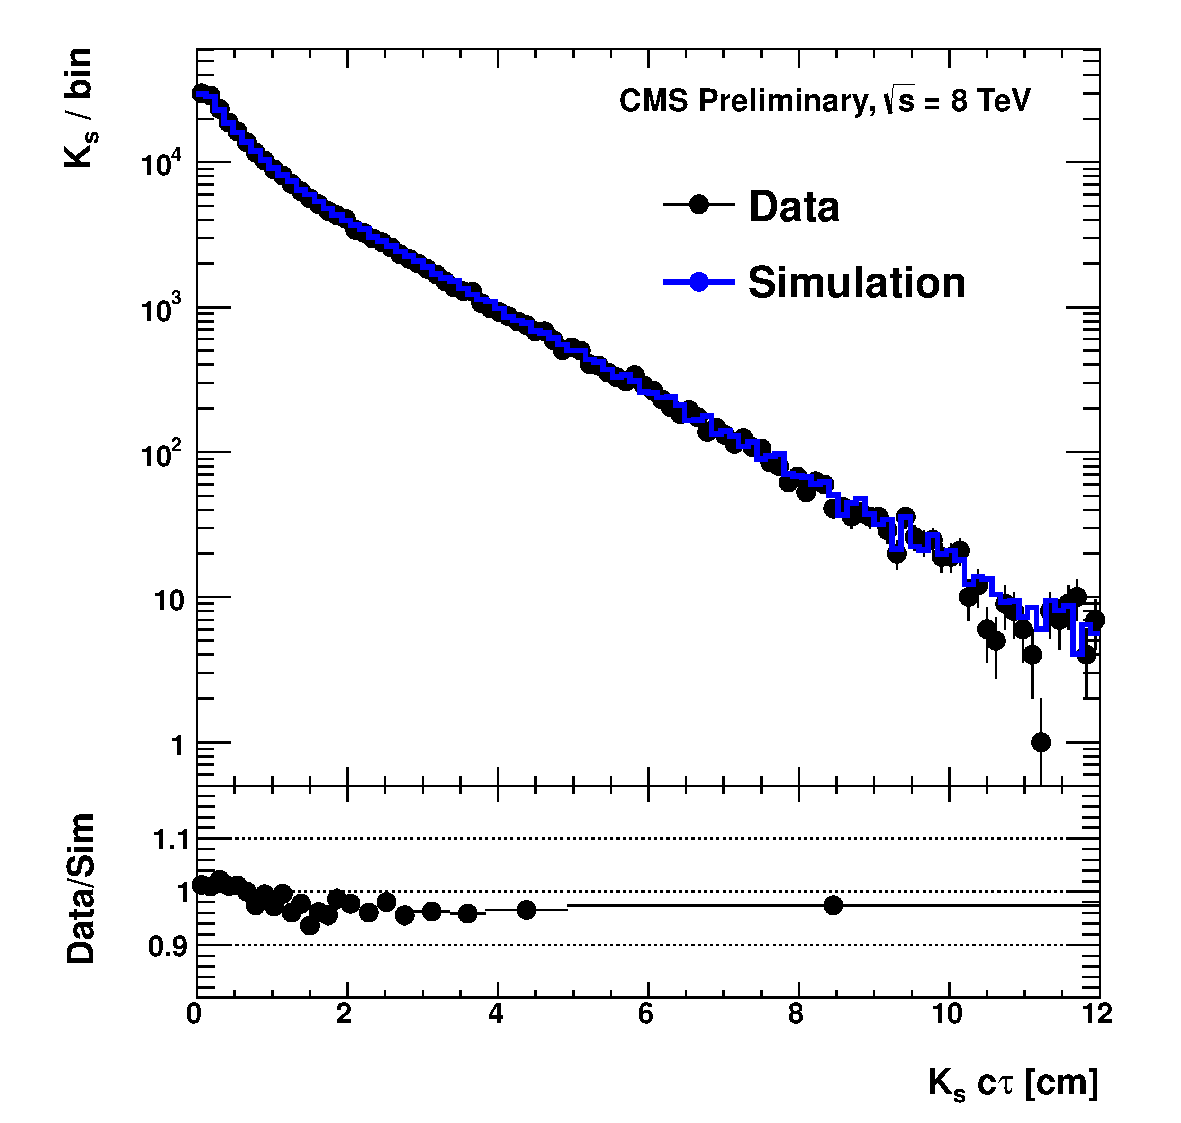
\includegraphics[width=0.49\textwidth]{plots/kshort/ksctau.pdf}
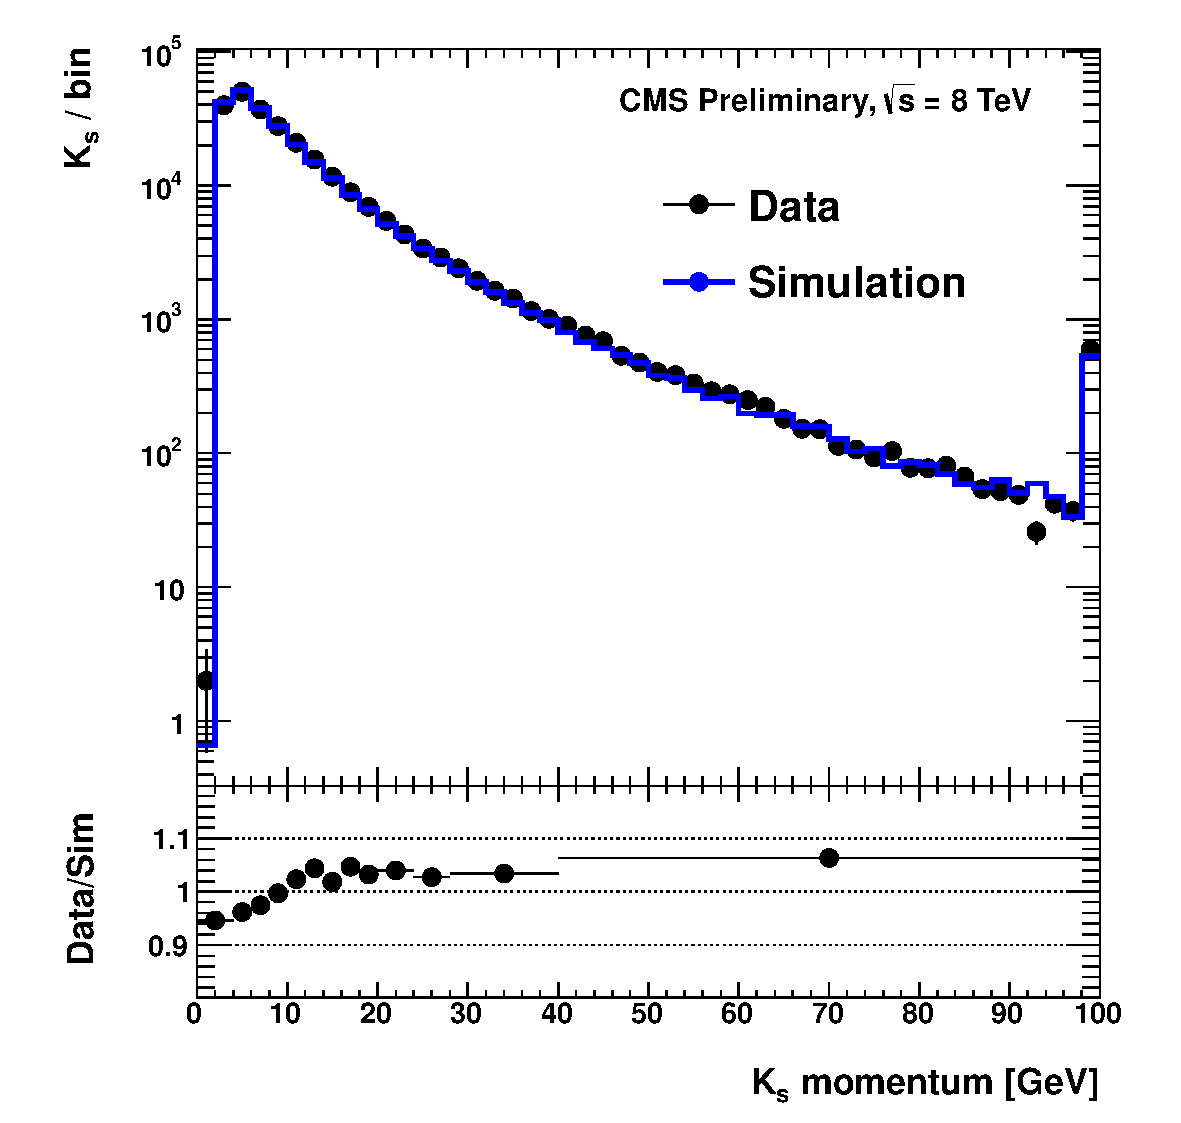
\includegraphics[width=0.49\textwidth]{plots/kshort/ksp.pdf}
\caption{Proper lifetime and momentum distributions of the \Kshort candidates in data and simulation. \label{fig:ksctau}}
\end{figure}

The proper lifetime and momentum distributions of the \Kshort candidates are
shown in Figure \ref{fig:ksctau}, while
Figure \ref{fig:ksdisplacement} shows the two and three dimensional decay lengths and track impact
 parameter distributions for data and simulation.  
 A good agreement between data and simulation is found, with simulation
 deviations not exceeding 10\%.   

\begin{figure}[htbp]
\centering
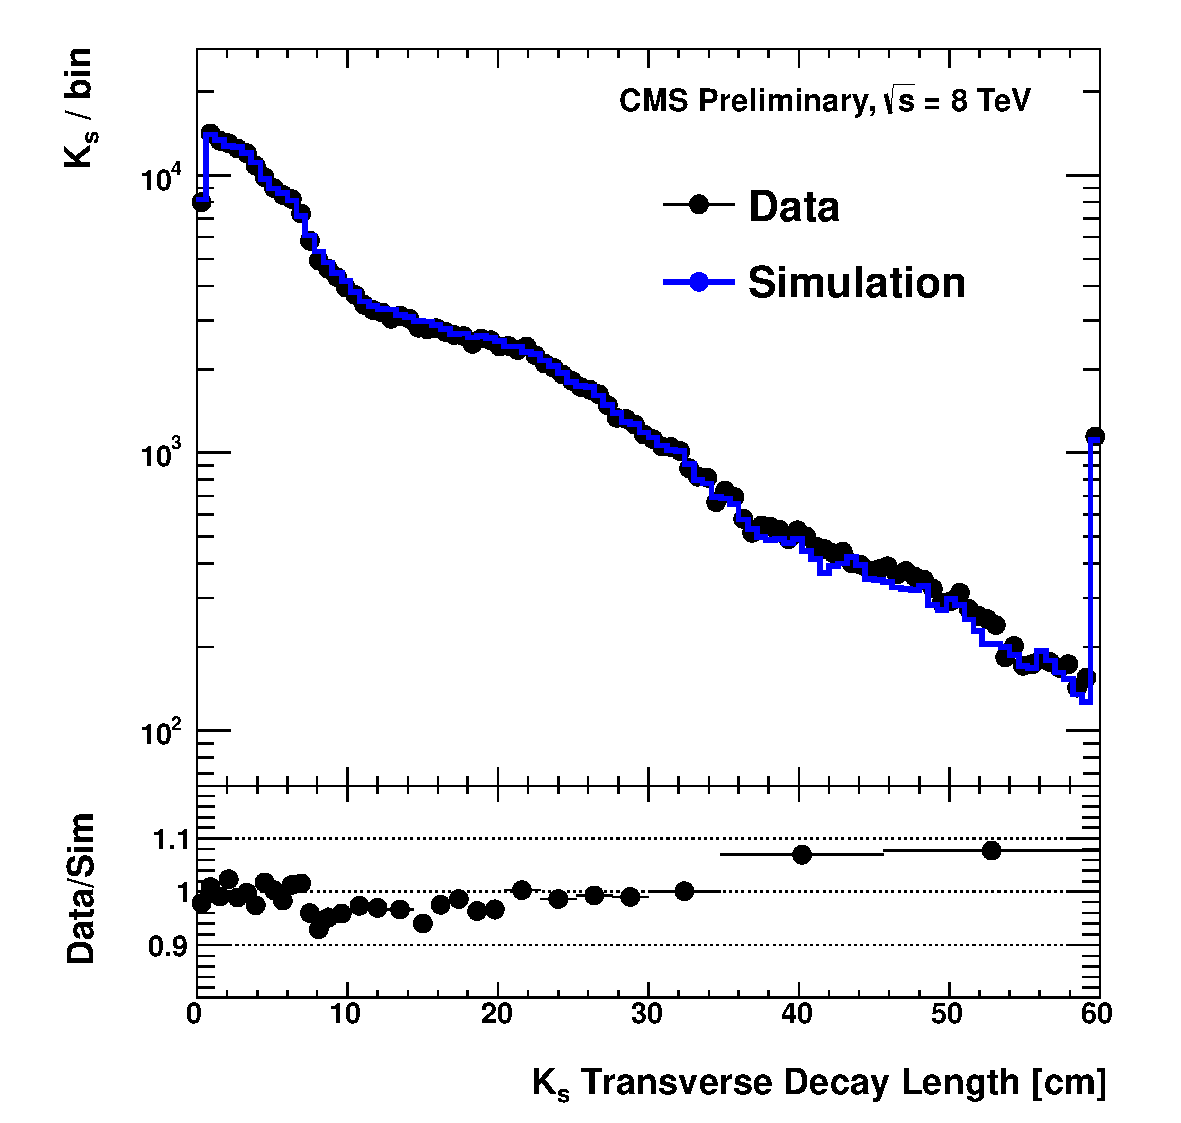
\includegraphics[width=0.49\textwidth]{plots/kshort/kslxy.pdf}
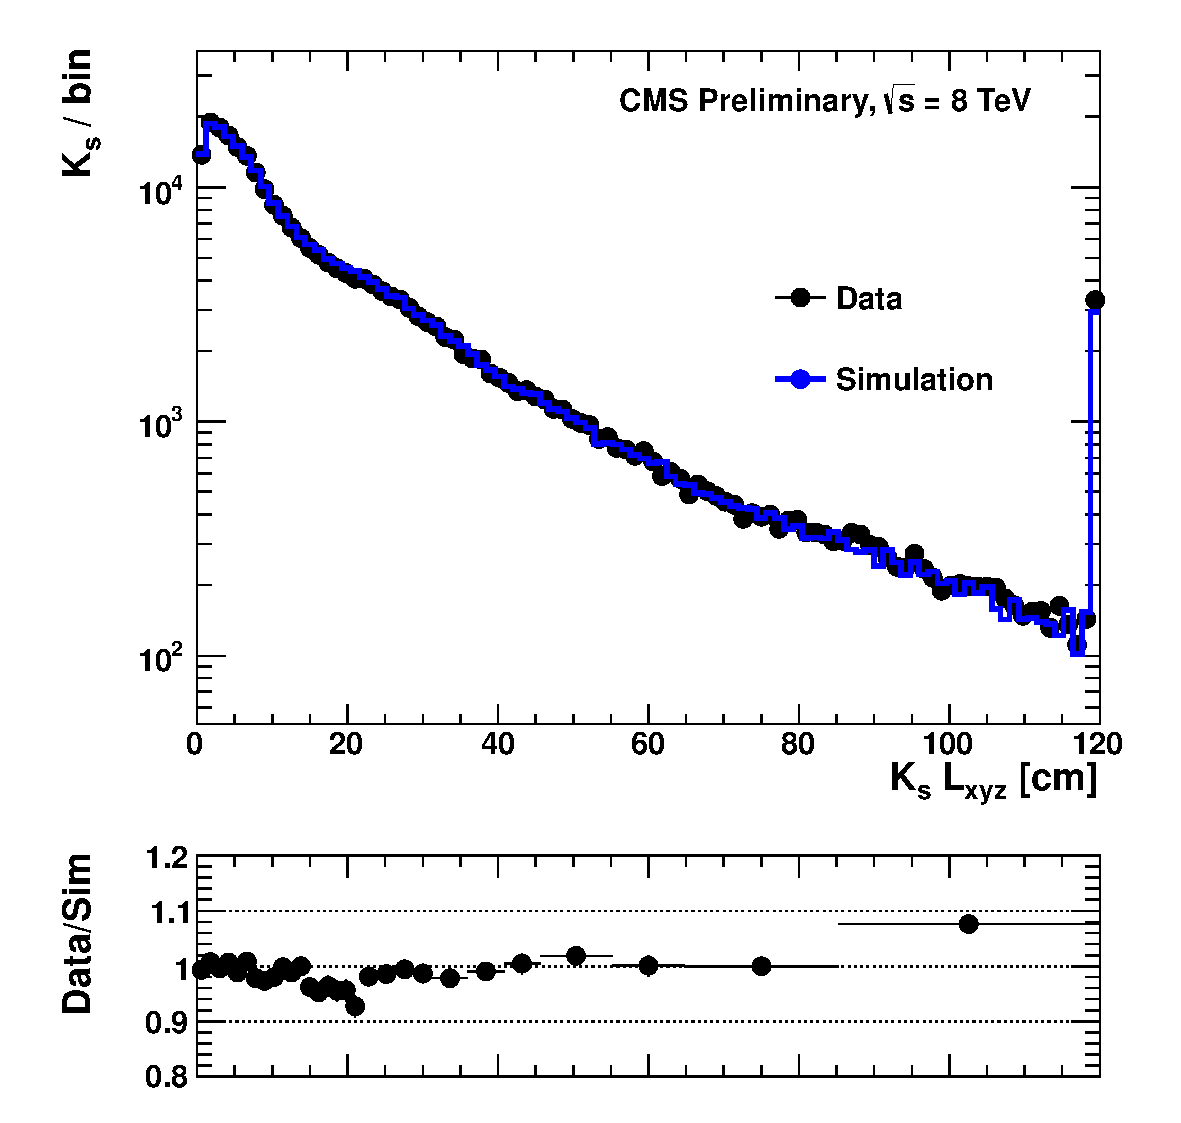
\includegraphics[width=0.49\textwidth]{plots/kshort/kslxyz.pdf}\\
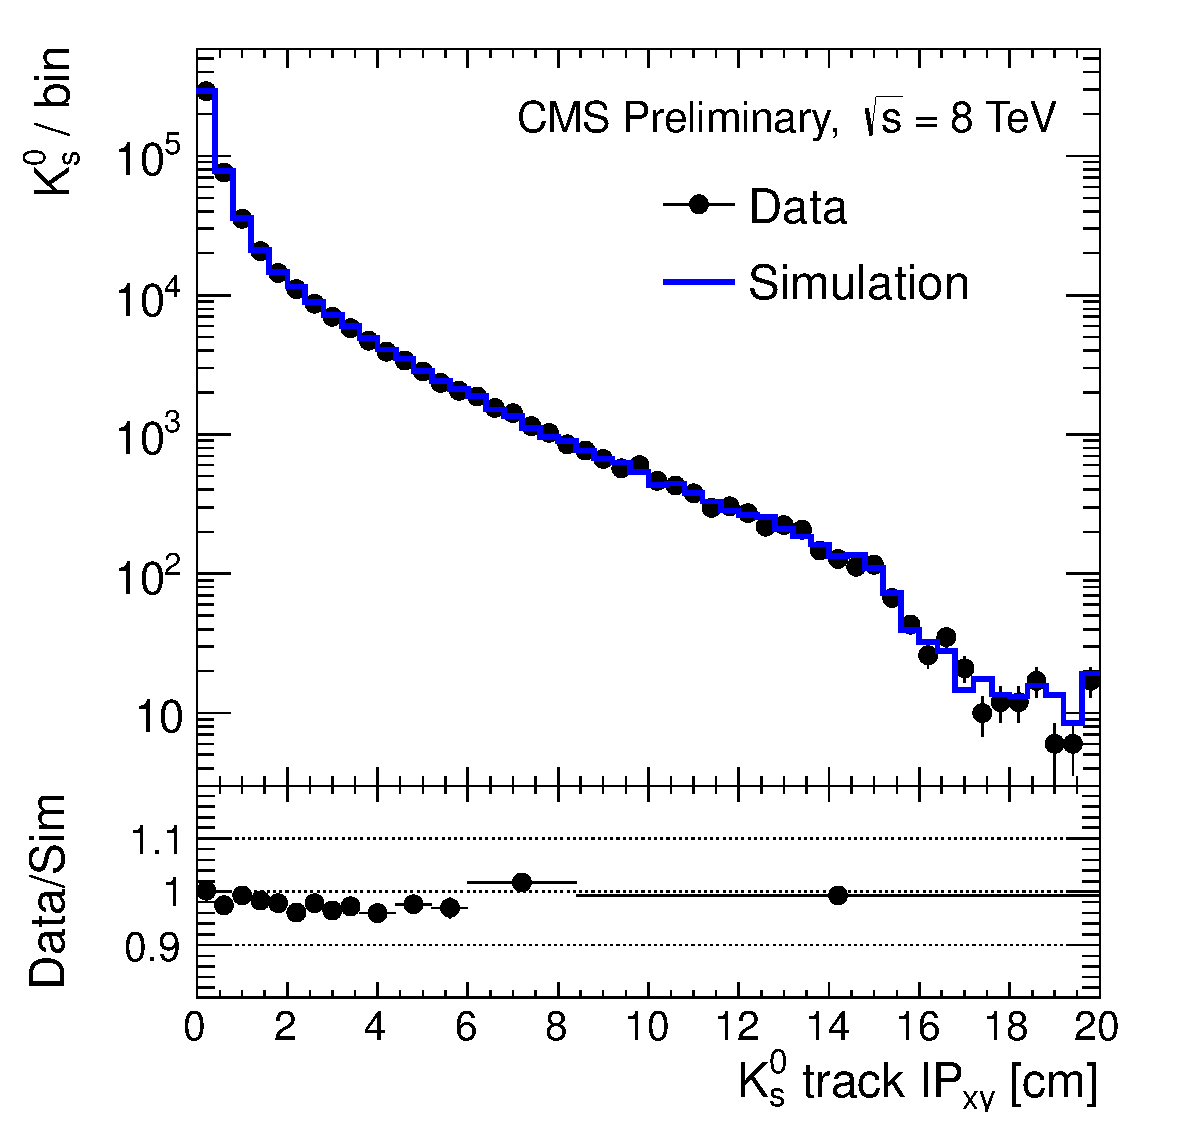
\includegraphics[width=0.49\textwidth]{plots/kshort/kstrkip2d.pdf}
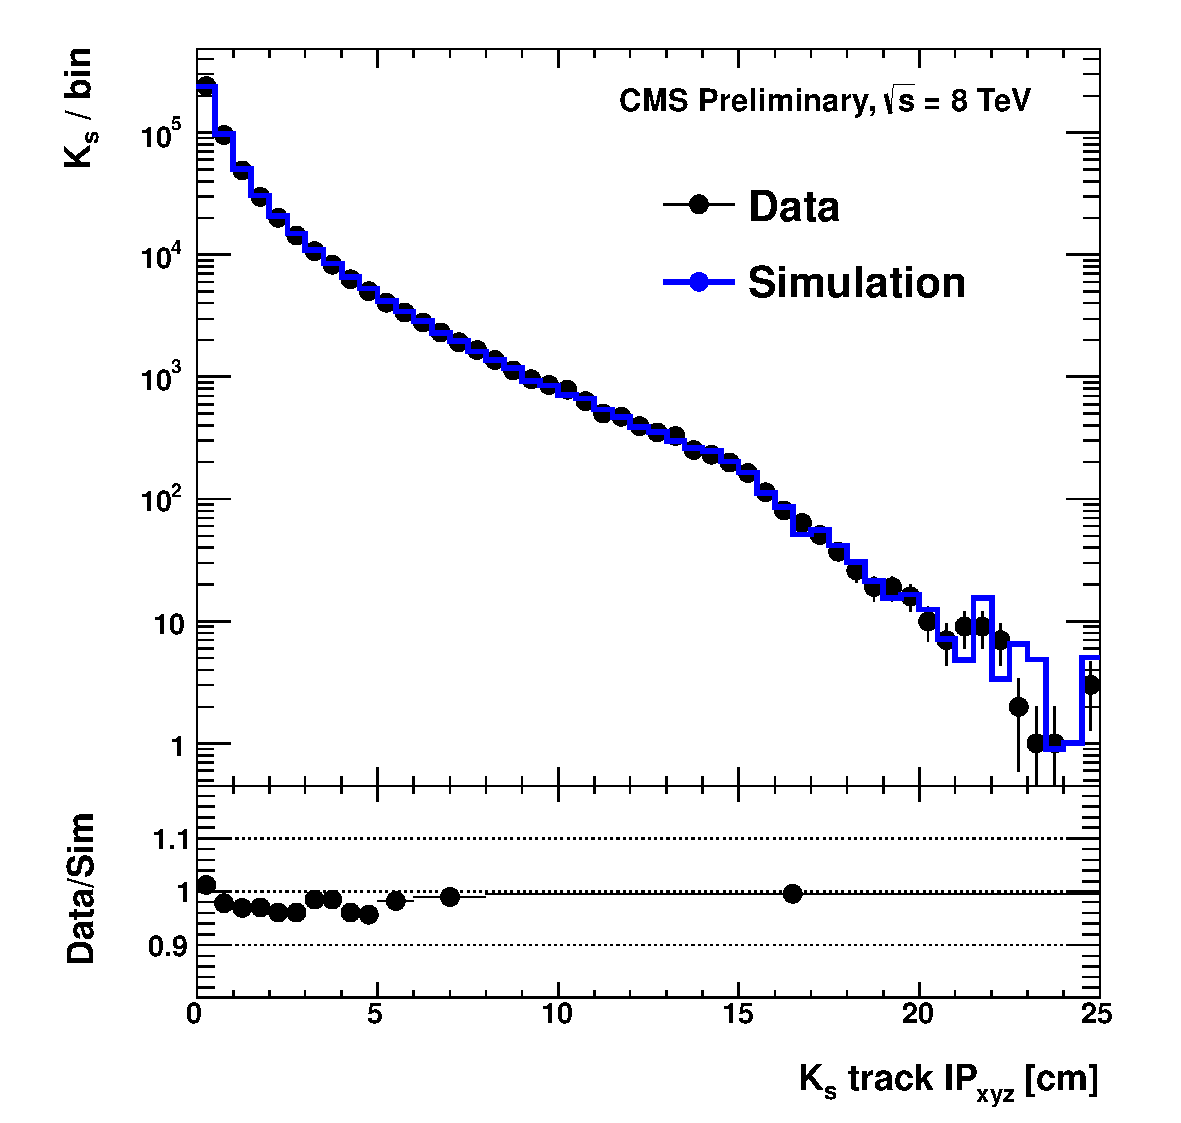
\includegraphics[width=0.49\textwidth]{plots/kshort/kstrkip3d.pdf}\\
\caption{Two-dimensional (top-left) decay length, three-dimensional decay length (top-right), two-dimensional track impact parameter (bottom-left) and three-dimensional track impact parameter (bottom-right) distributions 
of the \Kshort candidates in data and simulation. \label{fig:ksdisplacement}}
\end{figure}

The average number of 
reconstructed \Kshort candidates as a function of pile-up is presented in Figure \ref{fig:kspileup}. 
The decrease of tracking efficiency is found to be faster in data compared to simulation, while the 
effect is not bigger than 5\%.

\begin{figure}[htbp]
\centering
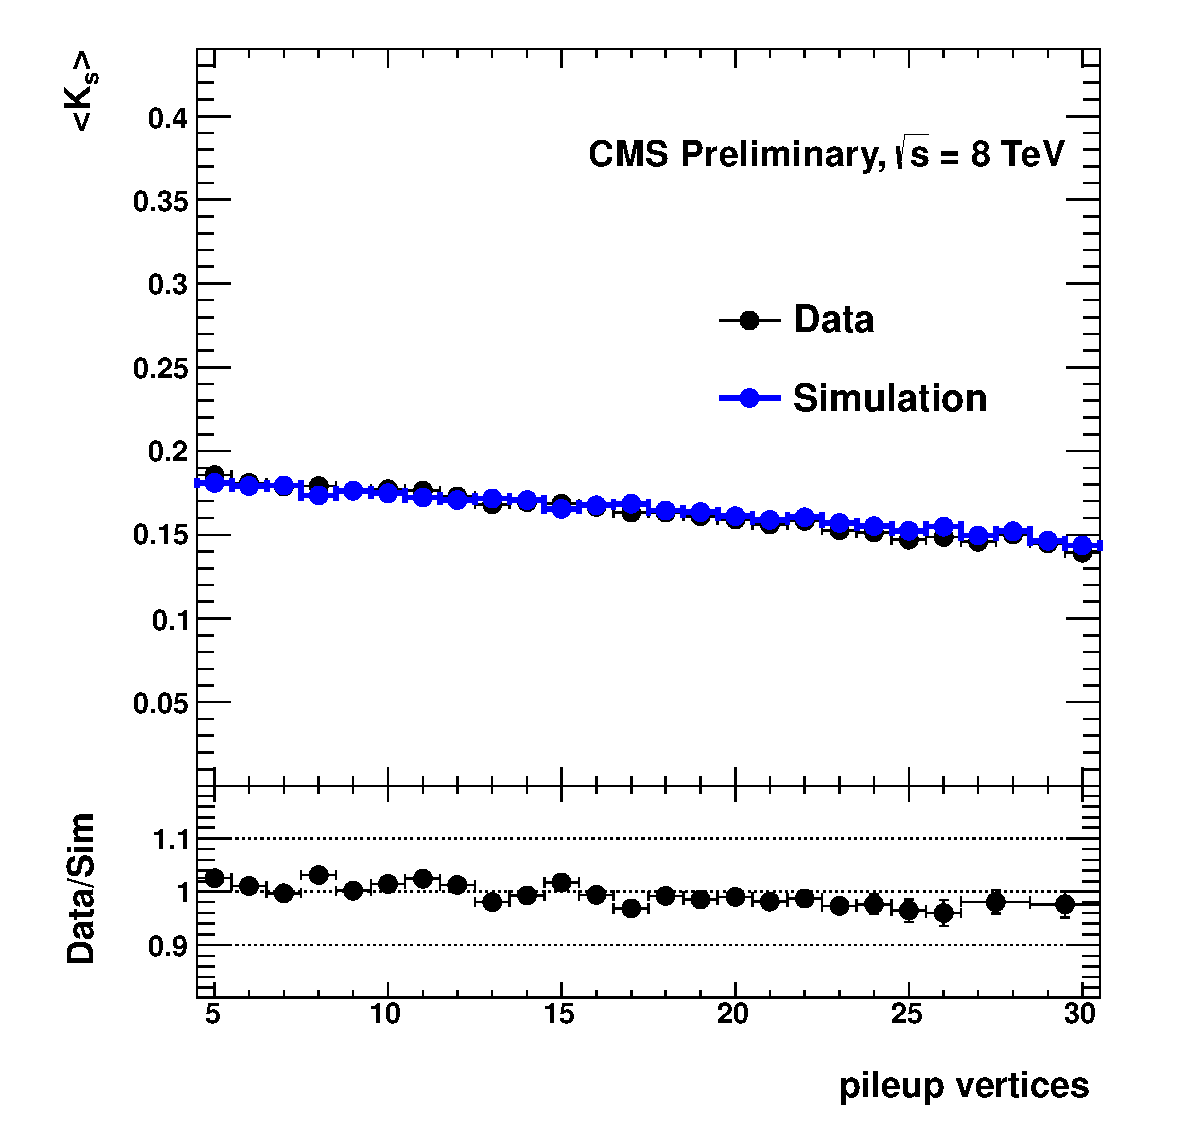
\includegraphics[width=0.49\textwidth]{plots/kshort/effnPV.pdf}
\caption{Average number of reconstructed \Kshort candidates as a function of number of primary vertices in data and simulation. \label{fig:kspileup}}
\end{figure}

The \Kshort reconstruction efficiency is proportional to the single track reconstruction efficiency squared, 
therefore the deviations between data and simulation of \Kshort distributions can be translated to twice smaller 
deviations in the single track reconstruction efficiency. We conservatively adopt the largest deviation 
of 10\% as the systematic uncertainty on the \Kshort efficiency and therefore a 5\% systematic on the 
single track reconstruction efficiency. 

\subsubsection{Impact on the signal reconstruction efficiency}

We examine the effect of tracking efficiency systematic uncertainty by removing 5\% of the displaced tracks 
 and repeating the signal reconstruction procedure.
For all signal models the reconstruction efficiency is lowered by up to 4\% which we adopt as our reconstruction
efficiency systematic related to displaced tracking efficiency.  

\subsection{Track missing hits}

In the pre-selection criteria the tracks in the displaced dijet vertex are required to have on average
 less than 2 missing hits behind the vertex position. The efficiency of this requirement is above 98\% 
for the simulated signal dijets as shown in Table \ref{tab:seleff}. 
The number of missing measurements depends on the number of tracking modules which are capable of providing
valid hits along the path of each track, which may not be properly simulated as the overall number of 
not functional modules in data changes over the data taking period. We study the average number of missing
hits behind the vertex position in a control sample of prompt dijets in data and simulation. We apply the
analogous selection criteria which are applied to the signal dijets,
 while omitting the requirements on prompt tracks and vertex displacement. Figure \ref{fig:misshits} presents
the average number of missing hits behind the vertex position per track for prompt dijets in data and simulation.

\begin{figure}[htbp]
\centering
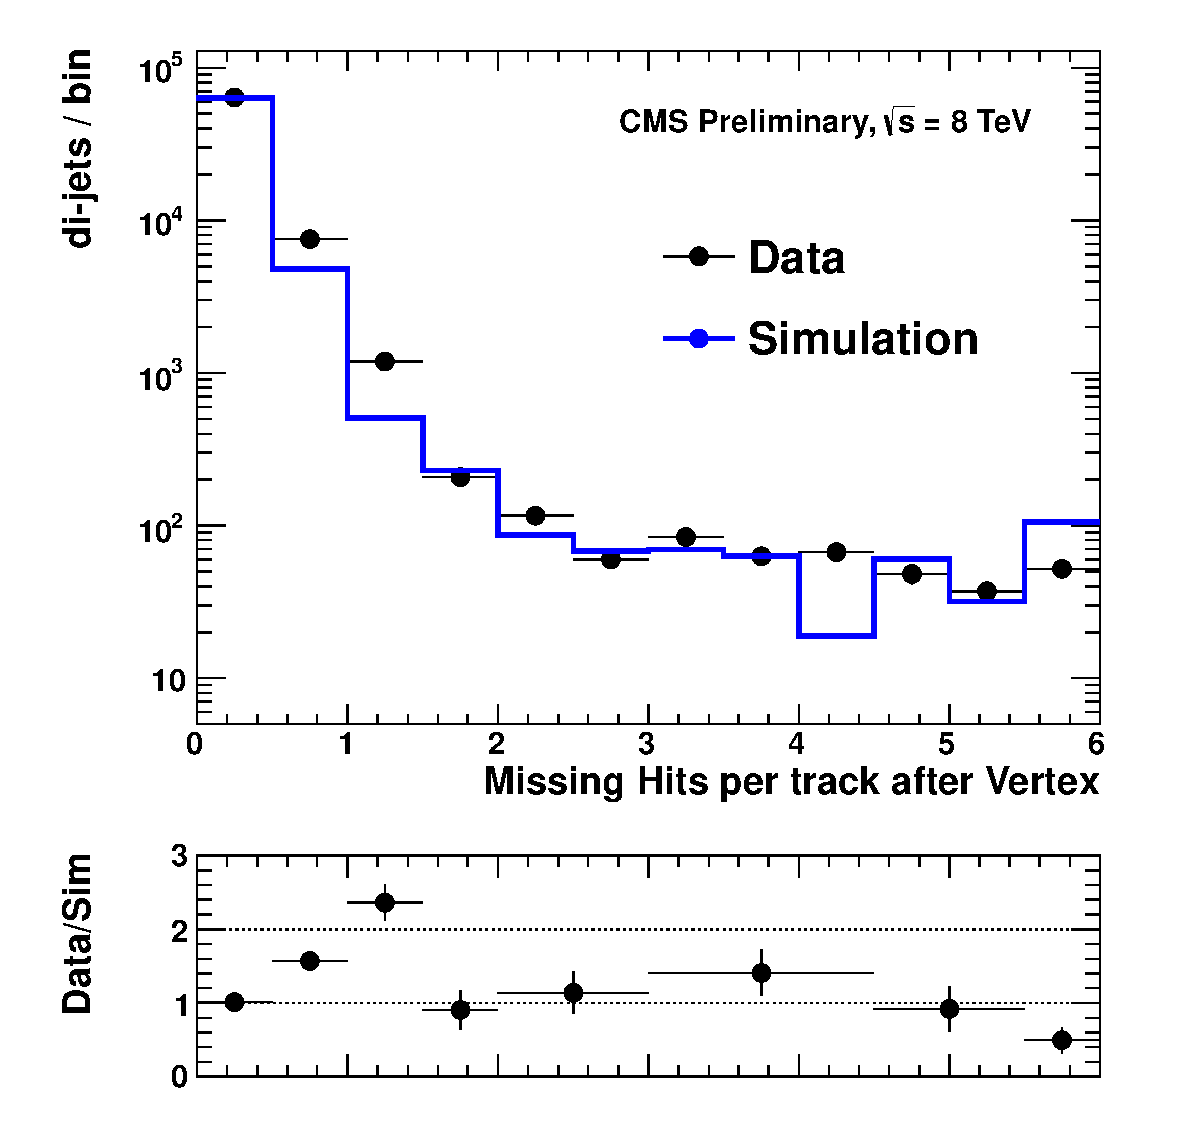
\includegraphics[width=0.49\textwidth]{plots/misshits/misshits.pdf}
\caption{Average number of tracker missing hits behind vertex position per track for prompt dijets
in data and simulation.\label{fig:misshits}}
\end{figure}

There are more missing hits observed in data, however the requirement of less than 2
missing hits on average is 98\% efficient in both data and simulation. Given the agreement in the efficiency
of this selection we do not assign additional systematic uncertainty. 

\subsection{Jet energy scale}
\label{subsec:jessys}

In CMS reconstruction the jet energies are determined by applying a set of corrections.
 The systematic uncertainties on the corrections are also provided. The uncertainties vary as a function
 of jet $p_T$ and $\eta$ and are different depending on the jet algorithm. Therefore, the effect of these
uncertainties on the signal reconstruction efficiency needs to be evaluated by applying variations to individual 
jets. In the event selection, described in Section \ref{subsec:selection},
 we use the jet energy information in the following criteria:
\begin{itemize}
\item $H_T>$325\GeV - using ak5Calo jets with $p_T>$40\GeV and $|\eta|<3$;
\item $p_T>$60\GeV for both jets of the di-jet candidate - here ak5PF jets within $|\eta|<2$ are used.  
\end{itemize}    

We determine the systematic uncertainty due to jet energy scale by shifting all relevant jet energies by 
their individual uncertainties up and down. Additionally, we assume that uncertainties for the two  
 jet algorithms, ak5Calo and ak5PF, are correlated, 
since they both use energy information from the calorimeters. The systematic 
difference in signal reconstruction efficiency upon jet energy scale variations is presented in Table
\ref{tab:jessys}. For \Higgs mass of 1000 \GeV the uncertainty is negligible, while for lower masses
of the \Higgs the systematic effect is below 5\%. 


%For mass of 400 \GeV the 
%difference between signal models with \X mass of 50 \GeV and 150 \GeV comes from the fact of overall 
%underestimation of the total $H_T$ for \X of mass 150 \GeV. The mean $H_T$ for this sample falls below 
%325 \GeV, which is used as an offline cut, therefore making the efficiency more sensitive to jet energy scale
%variations. The underestimation of jet energies for \X of mass 150 \GeV is due to the fact
%of signal jets being relatively wide. In such a scenario a 0.5 cone algorithm 
%does not contain all of the jet constituents, which results in an underestimate of its energy. 
%The effect of $H_T$ underestimation for \X mass of 150 \GeV does not depend on the \X particle mean lifetime.
 

\begin{table}[htbp]
\centering
\caption{Signal reconstruction efficiency bias due to jet energy scale uncertainties. \label{tab:jessys}}
\begin{tabular}{llc}
\hline
$M_{\Higgs}$ [\GeV] & $M_{\X}$ [\GeV]  & $\Delta\epsilon$ \\
\hline
200 & 50 & 4.4\% \\
400 & 50 & 2.7\% \\
400 & 150 & 4.8\% \\
1000 & 150 & 0.03\% \\ 
1000 & 350 & 0.02\% \\
\hline
\end{tabular}
\end{table}

\subsection{Jet momentum bias}
\label{subsec:ptbias}

\X boson jets originate at transversely displaced locations which leads to two effects that affect the jet 
momentum determination:
\begin{itemize}
 \item skewed approach angle at the calorimeters face. This effect is a result of the displacement 
of the jet production point combined with the opening angle of the \qq pair.
If the angle is large, the jet particles pass sideways through the calorimeters 
 which results in a geometrical bias of the individual
particles momentum and therefore the entire jet momentum;  
 \item reduced tracking efficiency for tracks originating far from the interaction point. This effect
is applicable only to Particle Flow jets which employ the tracking information, while it is not relevant for the 
Calo jets. In the Particle Flow algorithm when charged particles
are not reconstructed as tracks, they are assumed to be neutral particles, therefore the jet 
charged energy fraction is underestimated in favor of the neutral energy fraction. 
The calorimeter response to charged and neutral particles is different,
therefore the mis-measured energy fractions lead to biased jet energy corrections.
\end{itemize}
Figure \ref{fig:jetbias} shows the bias (points) and the resolution (error bars) of the signal jets $p_T$ 
, reconstructed with the Particle Flow algorithm, as a function of the \X boson transverse decay length $L_{xy}$.

\begin{figure}[htbp]
\centering
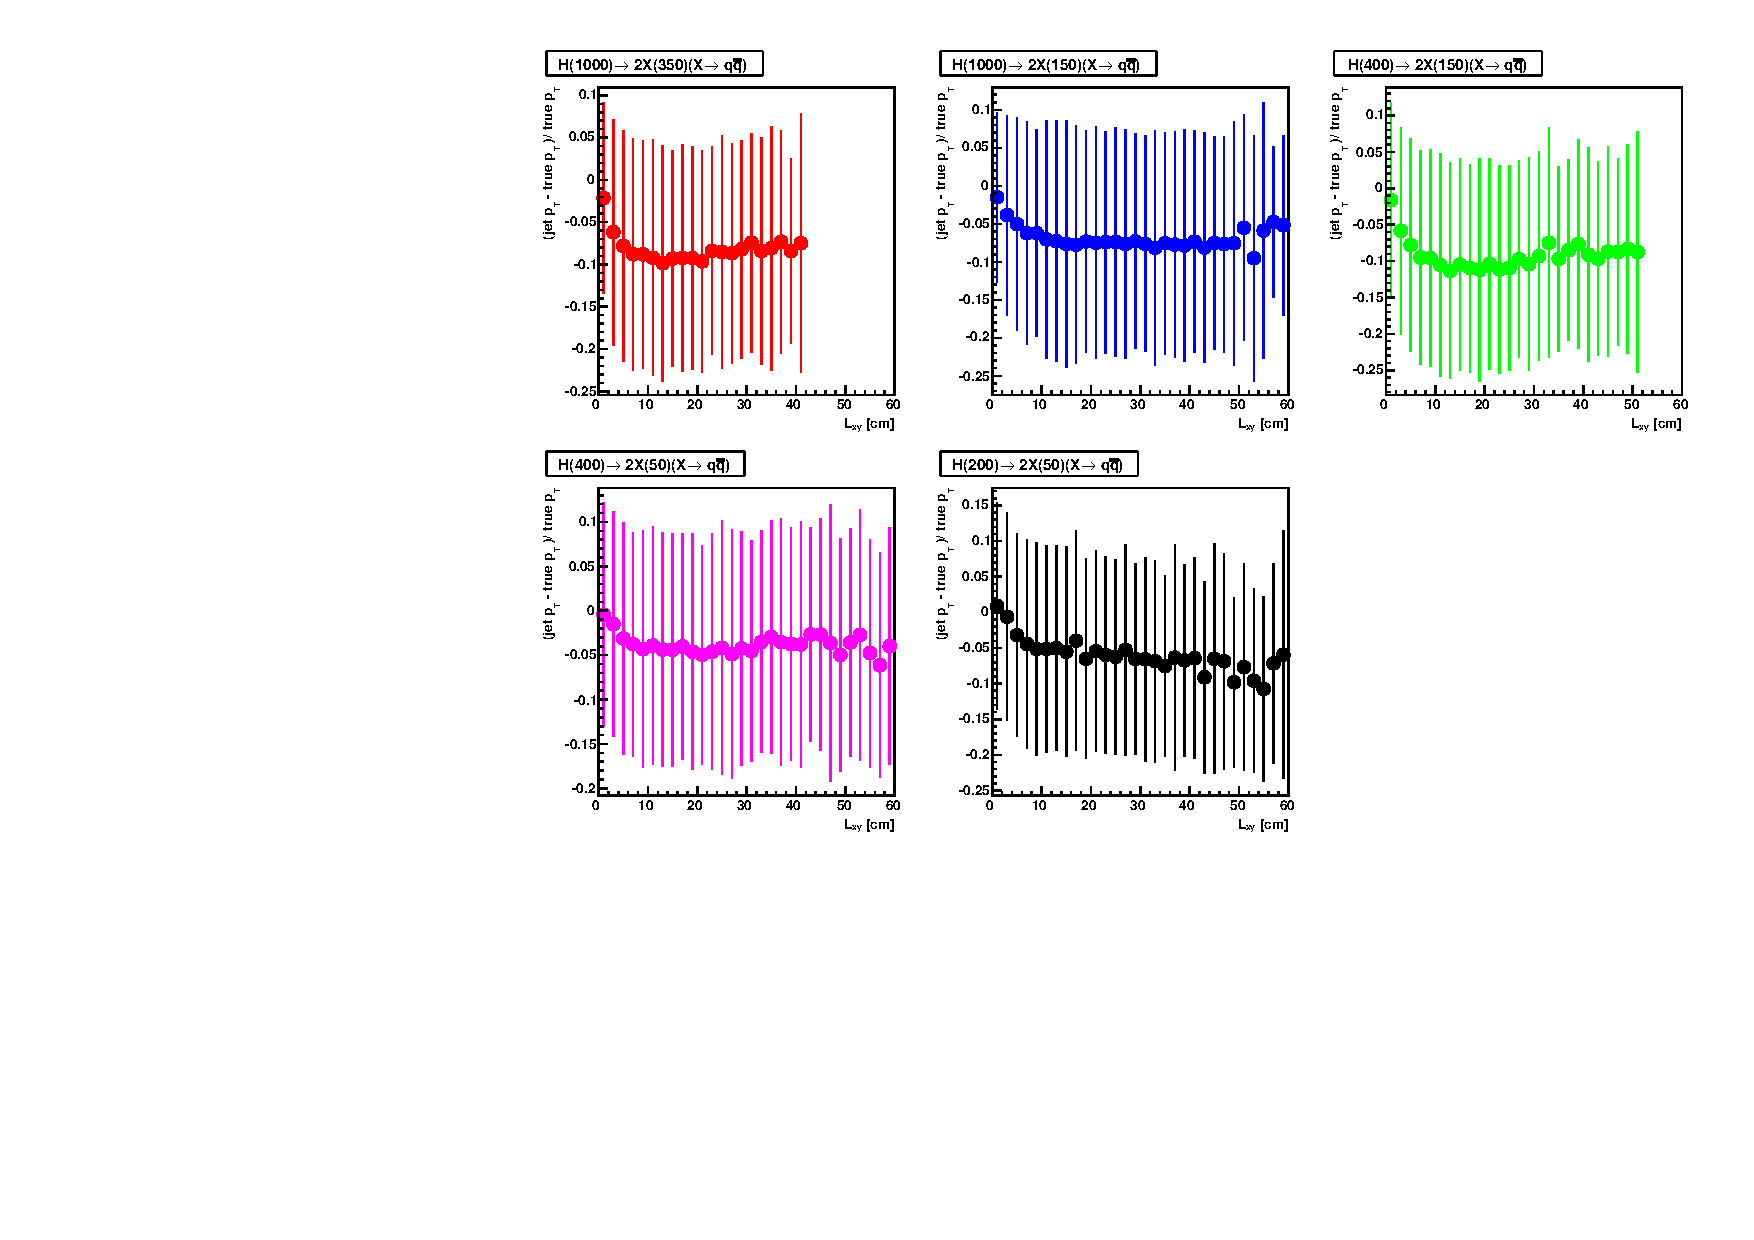
\includegraphics[width=0.99\textwidth]{plots/signal/biaslxy.pdf}
\caption{Signal jet $p_T$ bias and resolution as a function of the \X boson transverse decay length.\label{fig:jetbias}}
\end{figure} 
   
\begin{figure}[htbp]
\centering
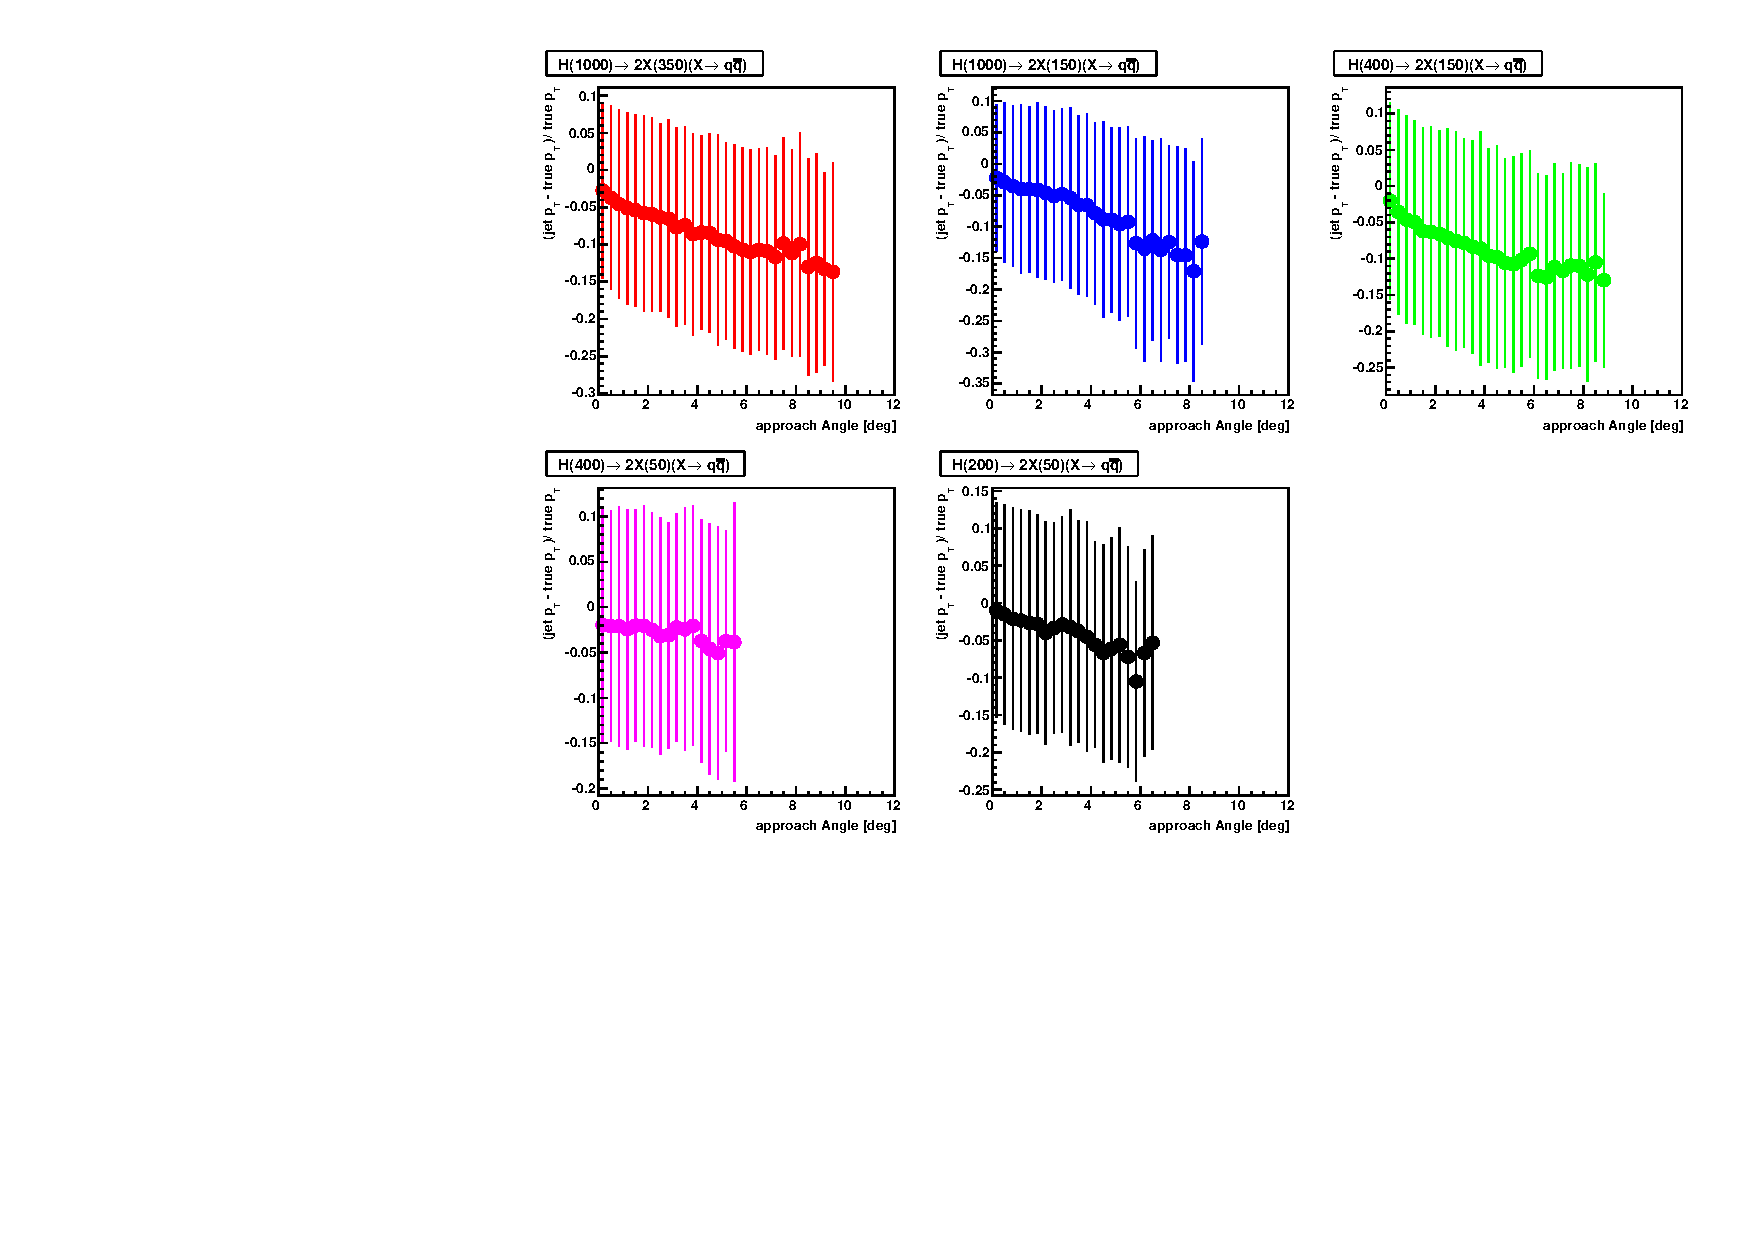
\includegraphics[width=0.99\textwidth]{plots/signal/biasapproachAngle.pdf}
\caption{Signal jet $p_T$ bias and resolution as a function of the jet approach angle at the calorimeters.\label{fig:jetbiasAngle}}
\end{figure} 

The jet momentum bias due to geometrical displacement is found to be up to -10\% for dijet candidates with transverse
decay lengths below 60\cm, while it is small for the prompt jets as expected. The level of the bias differs
depending on the signal mass point chosen, while the variation is related to the calorimeter approach angle
which is influenced by the opening angle of the \qq pairs.
The jet momentum bias as a function of the calorimeter approach angle is shown in Figure \ref{fig:jetbiasAngle}.
If the jet approach angle is restricted to below one degree, the jet momentum bias is found to be reduced by half.
 Therefore, the two effects related to tracking efficiency and skewed approach angle contribute to the 
momentum bias in approximately the same amounts.

We do not assign a systematic uncertainty related to the jet momentum bias arising from the skewed approach angle 
at the calorimeters under the assumption that the detector geometry is well described in the MC simulation.
In Section \ref{subsubsec:pitrkeff} we assign a 5\% systematic uncertainty on single track efficiency for 
displaced tracks. We therefore study a 5\% variation of the jet charged energy
fraction and its impact on the signal reconstruction efficiency with the results presented 
in Table \ref{tab:jetbias}. The variation is relevant only for selection criteria where Particle Flow jets
are used. 

\begin{table}[htbp]
\centering
\caption{Signal reconstruction efficiency bias upon a 5\% variation in the jet charged energy fraction.\label{tab:jetbias}}
\begin{tabular}{ccc}
\hline
  $M_{\Higgs}$ [\GeV] & $M_{\X}$ [\GeV] & $\Delta\epsilon$ \\
\hline
       ~200      &        50      &     4.9\%      \\
       ~400      &        50      &     4.5\%      \\
       ~400      &       150      &     3.6\%      \\
       1000      &       150      &     0.9\%      \\
       1000      &       350      &     0.5\%      \\
\hline
\end{tabular}
\end{table}

%\subsection{PDF systematics}
%\label{subsec:pdfsys}

%The signal Monte Carlo samples are generated using \PYTHIA. According to the recommendations on Parton Density
%Functions use at the LHC \cite{Bourilkov:2006cj}, the events are then re-weighted using 
%three PDF sets:
%\begin{itemize}
%\item CT10 - update of CTEQ6.6
%\item MSTW08
%\item NNPDF2.0
%\end{itemize}   
%The signal efficiency is calculated, where only kinematic selection criteria are applied, 
%namely the trigger, $p_T$ and pseudo-rapidity selections on
%the jets. These partial signal efficiencies are listed in Table \ref{tab:pdfsys}. Uncertainties on the efficiencies
% are determined from the systematic variation obtained with the listed PDF sets. 
%The relative uncertainty does
%not exceed 1\% for any considered signal model, therefore we adopt a 1\% systematic uncertainty as a conservative
%estimation of the PDF uncertainty for all signal models.
 

%\begin{table}[htbp]
%\centering
%\caption{Signal reconstruction efficiency for all simulated signal models, where only  the trigger, jet $p_T$ and 
%$\eta$ selections are applied. The uncertainties quoted on these numbers correspond to the systematic uncertainty on the PDF sets.\label{tab:pdfsys}}
%\begin{tabular}{llllc}
%\Higgs [GeV] & \X [GeV] & c$\tau$ [cm] & $\epsilon$ [\%] &  Relative Error [\%] \\
%\hline
%\hline
%200 & 50 & 2 & 2.3$\pm0.006$ & 0.3 \\
%200 & 50 & 20 & 3.1$\pm0.011$ & 0.4 \\
%\hline
%400 & 50 & 0.8 & 28.0$\pm0.19$ & 0.7 \\
%400 & 50 & 8 & 50.0$\pm0.4$ & 0.7 \\
%400 & 50 & 80 & 11.0$\pm0.11$ & 1.0 \\
%\hline
%400 & 150 & 4 & 38.0$\pm0.29$ & 0.8 \\
%400 & 150 & 40 & 43.0$\pm0.43$ & 1.0 \\
%400 & 150 & 400 & 9.3$\pm0.10$ & 1.0 \\
%\hline
%1000 & 150 & 1 & 75.0$\pm0.16$ & 0.2 \\
%1000 & 150 & 10 & 85.0$\pm0.30$ & 0.4 \\
%1000 & 150 & 100 & 23.0$\pm0135$ & 0.6\\
%\hline
%1000 & 350 & 3.5 & 91.0$\pm0.10$ & 0.1 \\
%1000 & 350 & 35 & 93.0$\pm0.11$ & 0.1 \\
%1000 & 350 & 350 & 34.0$\pm0.26$ & 0.8 \\
%\hline
%\end{tabular}
%\end{table}

\subsection{Effect of higher-order QCD corrections}
\label{subsec:isr}

As described in Section \ref{subsec:jessys} the signal reconstruction efficiency is sensitive to the jet energy
scale variations; in particular for signal models with \Higgs mass of 200 \GeV and 400 \GeV. 
Therefore, the signal reconstruction efficiency is also sensitive to the modelling of
 the Higgs $p_T$ spectrum, which may be in turn influenced by higher-order QCD corrections. 
To study this effect
we re-weight the \PYTHIA \Higgs $p_T$ spectrum from our signal samples to match the corresponding distribution
determined at NLO using \POWHEG \cite{Bagnaschi:2011tu}. For $M_{\Higgs}$ = 200 \GeV with $M_{\X}$ = 50 \GeV and for $M_{\Higgs}$ = 400 \GeV 
with $M_{\X}$ = 150 \GeV signal models this changes the efficiency by 20\% and 3\% respectively, while for
other signal models the corresponding change is below 1\%. 
Since the hidden valley signature is used as a benchmark
model, we do not incorporate this variation as an additional systematic uncertainty, but emphasize and quantify
the sensitivity of the reconstruction efficiency to higher-order QCD corrections.  

\subsection{Trigger Efficiency}
\label{subsec:trigeff}

The high level trigger used in the analysis, HLT\_HT300\_DoubleDisplacedPFJet60, has been emulated in all
 simulation samples. Trigger selection consists of several consecutive filters applied to each event, 
and the performance of each filter is studied individually in data and simulation with respect to 
the corresponding offline selection criteria. For studying each individual filter, events 
passing all trigger decisions 
are not used in order to avoid a possible bias with the signal sample. Individual filters and their efficiency are
described in the following sections.  

\subsubsection{Scalar sum of jets $E_T$}
\label{subsubsec:trigHT}
This trigger filter requires $H_T > $ 300\GeV. Its performance is studied using a lower threshold trigger which 
requires $H_T >$ 250\GeV. 
The HT250 trigger has been heavily prescaled in 2012 LHC run, therefore the integrated luminosity corresponds to only 8\pbinv. 
In both trigger calculation and offline reconstruction, calorimeter jets with $p_T>$40\GeV and $|\eta|<$3 are used
 for $H_T$ computation. 
Figure \ref{fig:effHT300} shows the trigger efficiency as a function of the offline $H_T$. 
The difference in performance between data and simulation can be inferred from the efficiency ratio 
shown at the bottom. The observed discrepancy in the turn-on curves close to the threshold is caused by the 
difference in Level 1 trigger seeds used in the simulation compared to data.
An offline selection on 
$H_T$ at 325\GeV is applied in the selection criteria. 
Above this value the differences in efficiency between data and simulation are up to
7\%. To account for these differences the simulation events are re-weighted to match the efficiency in data.
This re-weighting
lowers the signal efficiency by up to 2\% for all considered signal models. The systematic effects in the turn-on
curve shape are studied by re-weighting the simulation with data turn-on curves corresponding to
 different periods of the LHC data taking in 2012. The variations in efficiency are found consistent within 
less than 1\%, while we conservatively assign 1\% as a relative 
systematic uncertainty corresponding to this trigger filter.      

\begin{figure}[htbp]
\centering
 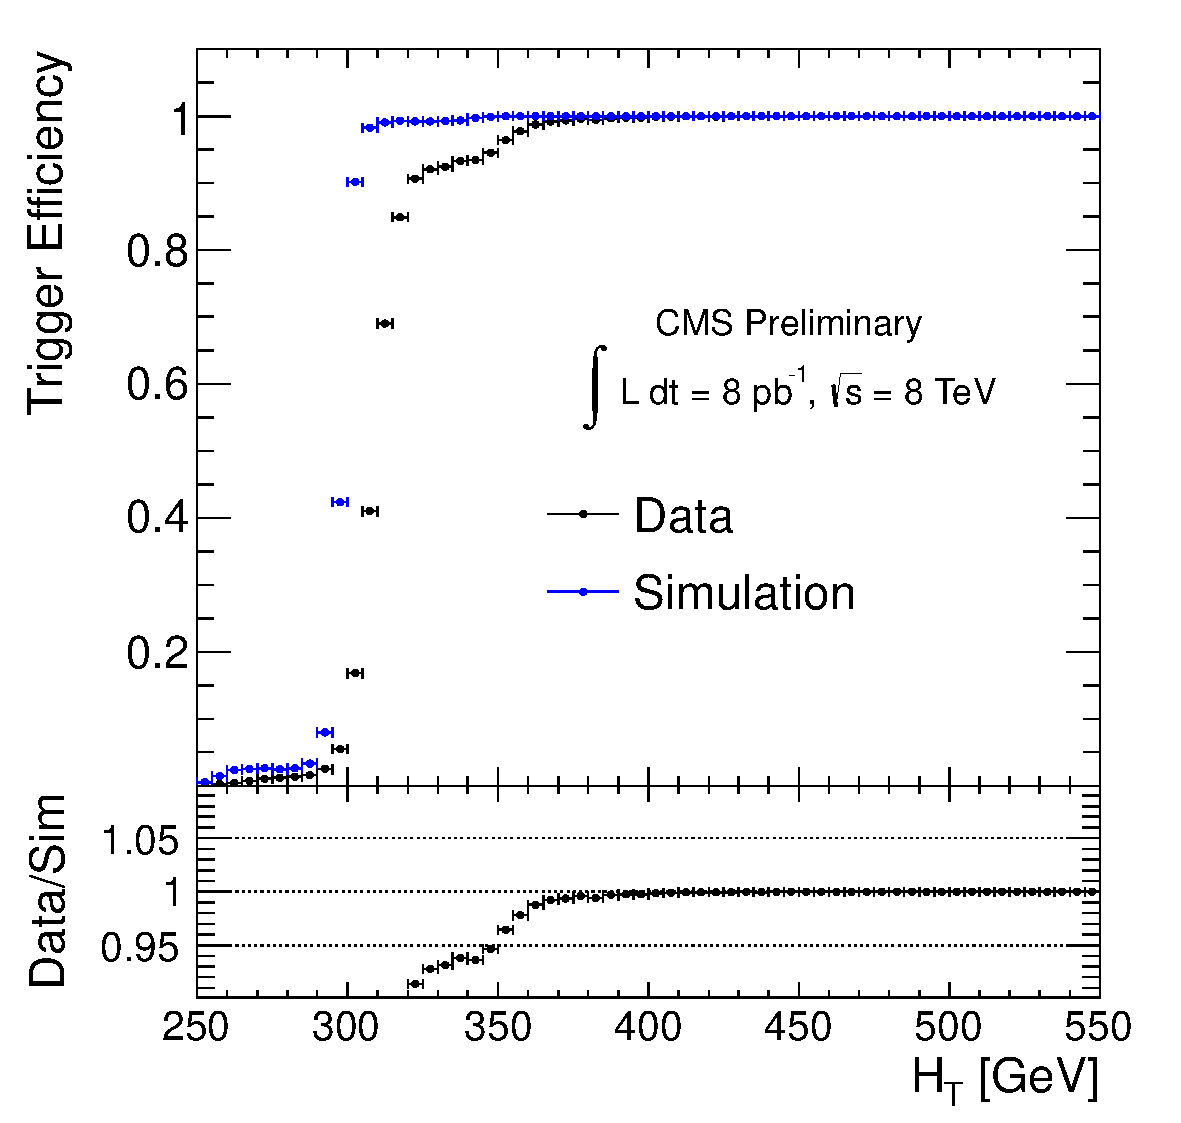
\includegraphics[width=0.49\textwidth]{plots/trigger/effHT300.pdf}
\caption{HLT\_HT300 trigger efficiency as a function of offline $H_T$ requirement. \label{fig:effHT300}}
\end{figure} 

\subsubsection{Two jets each with maximally 2 prompt tracks}
\label{subsubsec:trig2Trks}

This filter is analyzed with data passing the previous 
HT300 filter. Data collected by CMS with this trigger amounts to 17\pbinv.  While the filter in question
 requires at least two jets with $p_T>$ 60\GeV passing the requirement, it is sufficient to study
 only the efficiency
 of a single jet passing the filter with respect to number of prompt tracks computed offline.
 In both HLT trigger and offline
 reconstruction prompt tracks are selected as those with an impact parameter in 3 dimensions 
not bigger than 300$\mum$
 with respect to leading primary vertex. Figure \ref{fig:eff2Trks} shows the single jet efficiency of passing
 the requirement of maximally 2 prompt tracks as a function of the same variable computed offline.
 The trigger becomes efficient with number of offline prompt tracks less than 2. 
A drop in efficiency for 0 prompt tracks arises from a fact of different leading primary vertex assignment 
between HLT and offline reconstructions. 
In such a scenario a track may be assumed to be prompt at HLT and non-prompt
 in offline reconstruction or vice versa. 
  

\begin{figure}[htbp]
\centering
 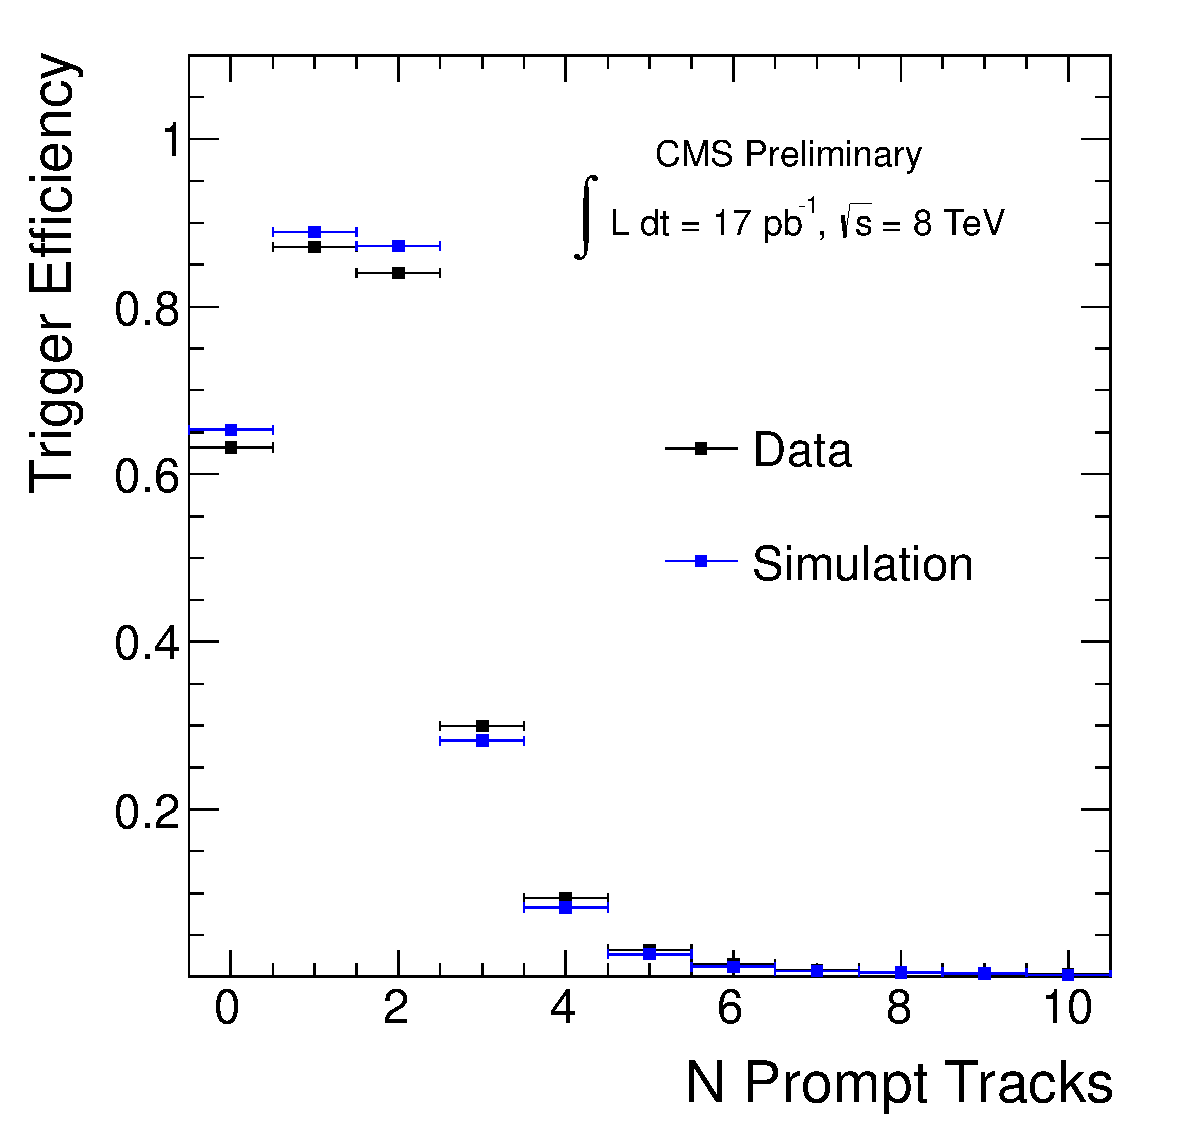
\includegraphics[width=0.49\textwidth]{plots/trigger/effHT300_2Trk_NPromptTracks.pdf}
\caption{Single jet efficiency for jets having maximally of 2 prompt tracks as a function of number of offline prompt tracks. \label{fig:eff2Trks}}
\end{figure}

The trigger efficiency for jets passing the offline selection of maximally 2 prompt tracks 
is plotted in Figure \ref{fig:eff2Trksptetaphi}
 as a function of $p_T$, $\eta$ and $\phi$. In order to determine the differences in performance 
between data and simulation the efficiency ratios are fitted with a zeroth order polynomial for each variable.
The fits yield a value of 97\% consistent within statistical uncertainties in $p_T$, $\eta$ and $\phi$,
 however with the $\chi^2$ per degree of freedom of the fits up to 4. 
The statistical uncertainties on individual points in the ratio histograms
are thus inflated by a factor of 2 and the ratios refitted.
 The overall correction is determined from the average of the fit values for
$p_T$, $\eta$ and $\phi$ with the result of 97\%. The systematic uncertainty on the ratio 
is assigned as the maximal
difference between the fit values within their statistical uncertainties with the result of 0.6\%.
Therefore, we assign an overall correction of 97\% with a conservative 1\% systematic uncertainty for 
each jet passing this trigger filter. 
 
 
\begin{figure}[!h]
\centering
 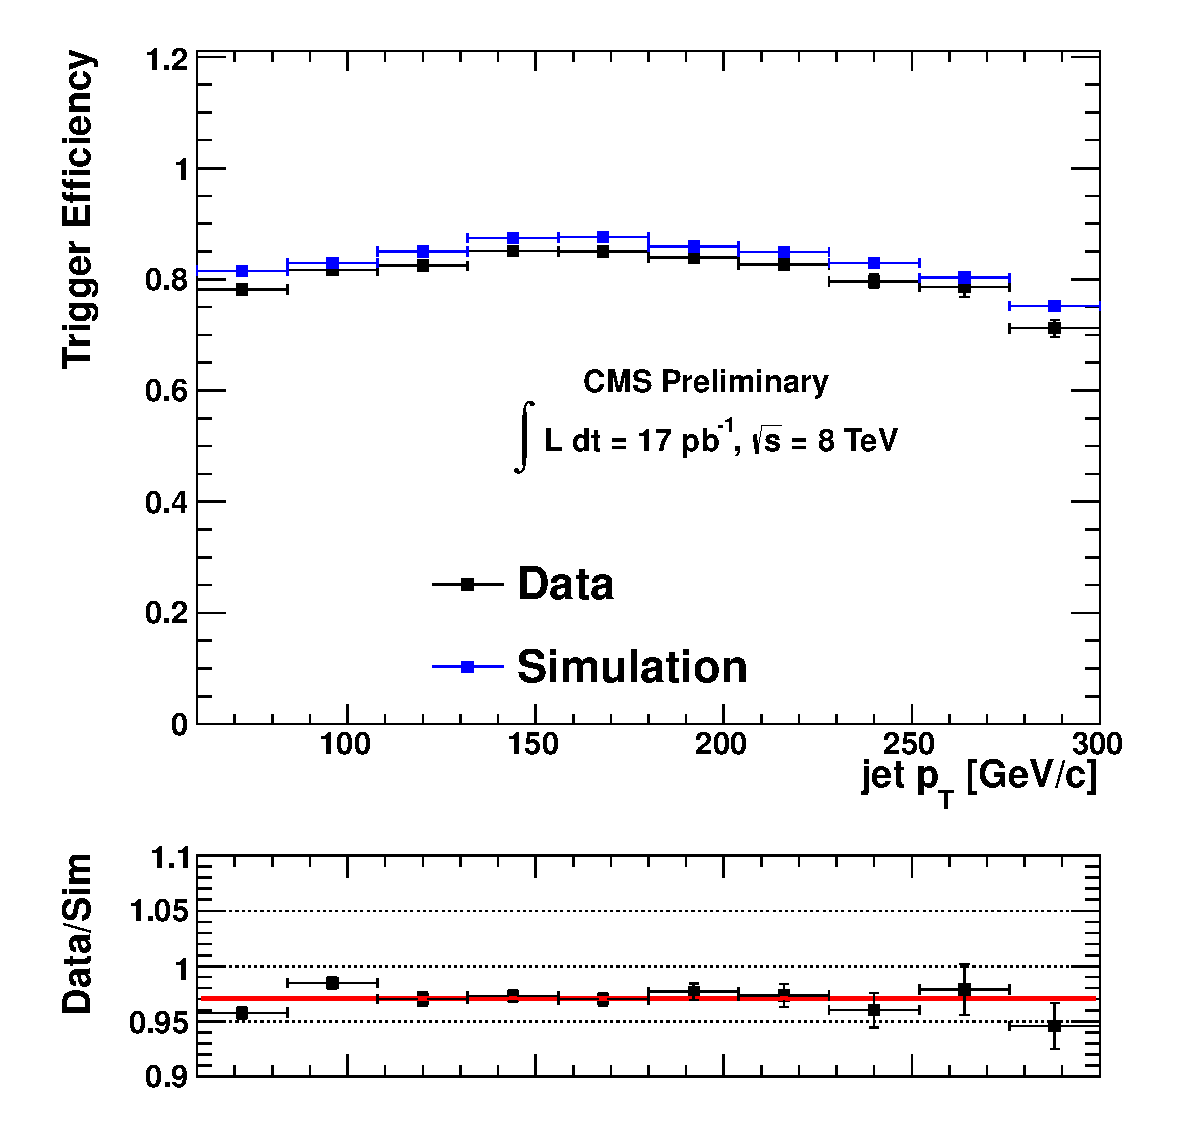
\includegraphics[width=0.32\textwidth]{plots/trigger/effHT300_2Trk_Pt.pdf}
 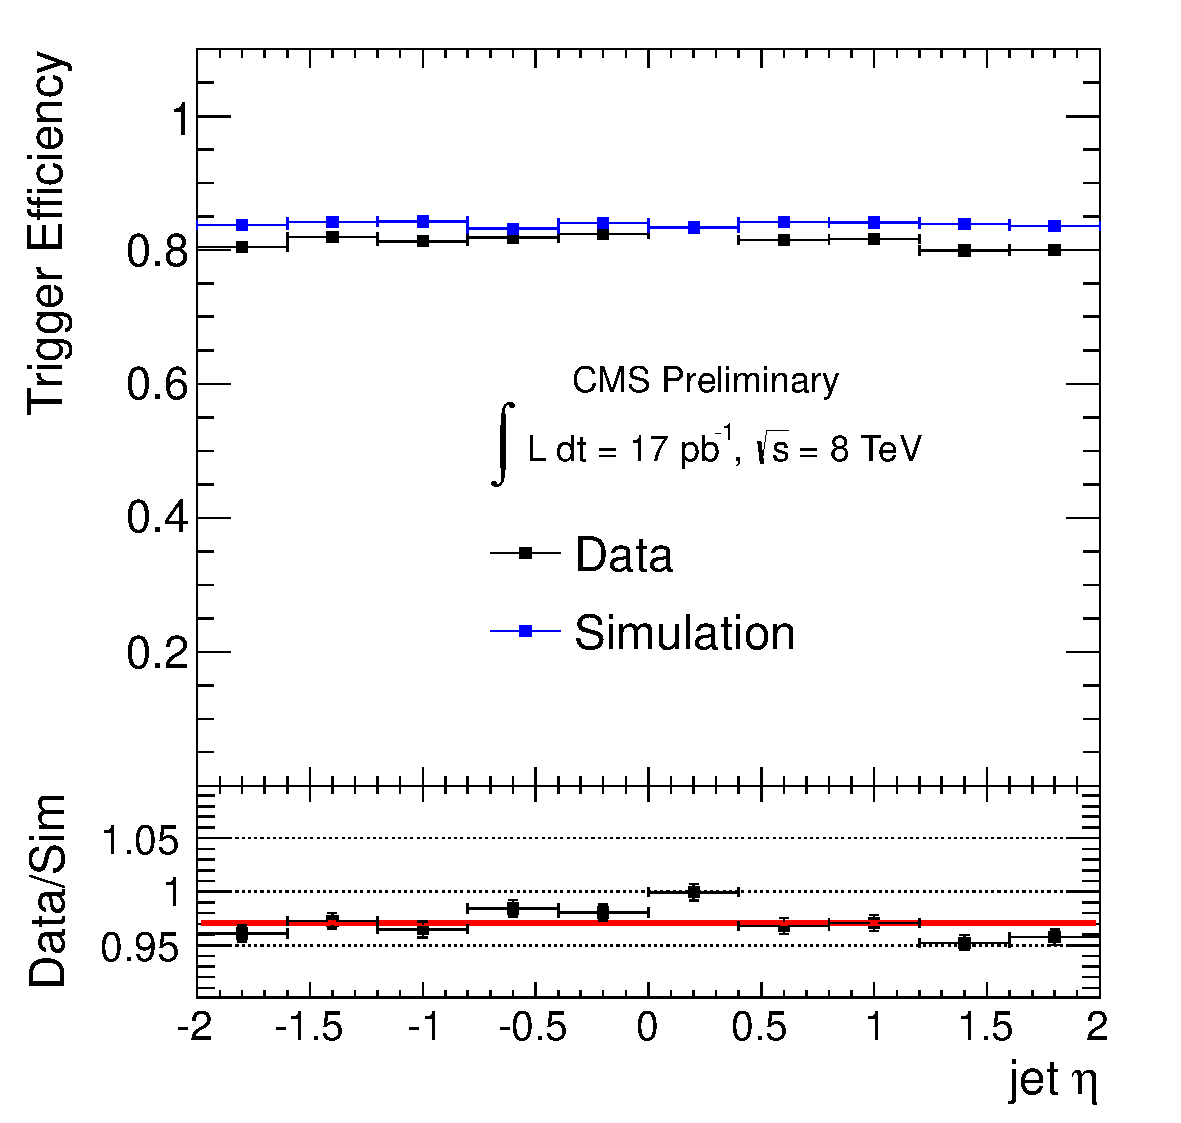
\includegraphics[width=0.32\textwidth]{plots/trigger/effHT300_2Trk_Eta.pdf}
 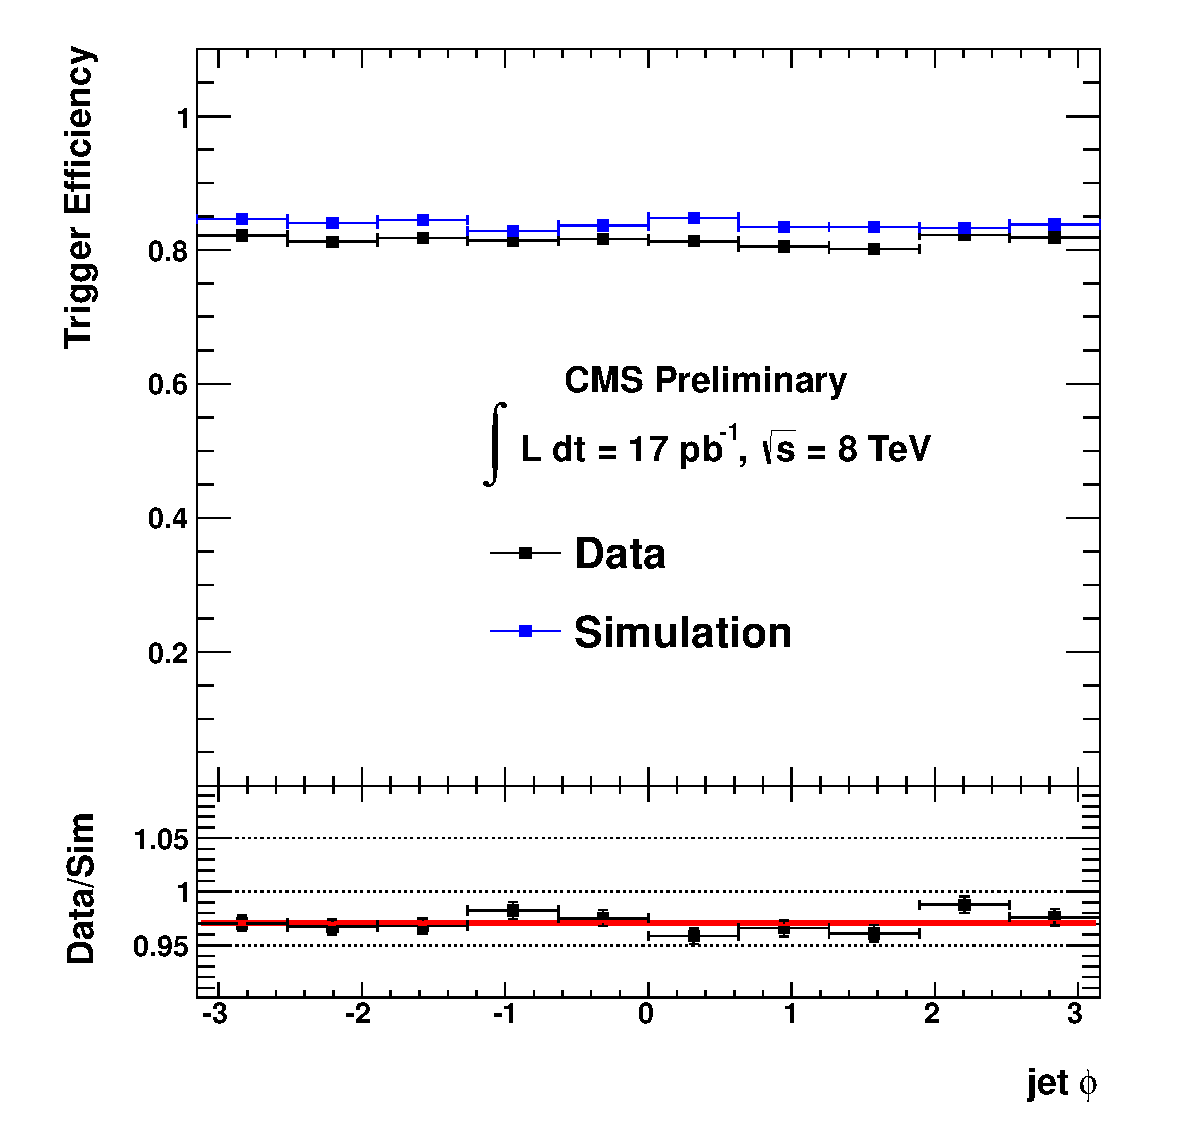
\includegraphics[width=0.32\textwidth]{plots/trigger/effHT300_2Trk_Phi.pdf}
\caption{Single jet efficiency as a function of jet $p_T$, $\eta$ and $\phi$ for jets with maximally 2 offline prompt tracks. \label{fig:eff2Trksptetaphi}}
\end{figure}

\subsubsection{Two jets with maximally 15\% of energy fraction carried by prompt tracks}
\label{subsubsec:trig2PF}

Similarly, we require both filters from Sections \ref{subsubsec:trigHT} and \ref{subsubsec:trig2Trks} 
to accept the event and examine a single jet efficiency with respect to prompt charged energy
 fraction computed offline. In this trigger step the prompt tracks are defined
 as those having the transverse impact parameter not bigger than 500$\mum$. 
Using transverse impact parameter
minimizes the sensitivity to additional pile-up interactions in the event. The size of the luminous region in 
the transverse plane is very small, about 30$\mum$, therefore the track promptness definition is general
and does not depend on the choice of the leading primary vertex. 
Trigger efficiency as a function of prompt energy fraction computed offline is shown in Figure \ref{fig:eff2PF}.

\begin{figure}[htbp]
\centering
 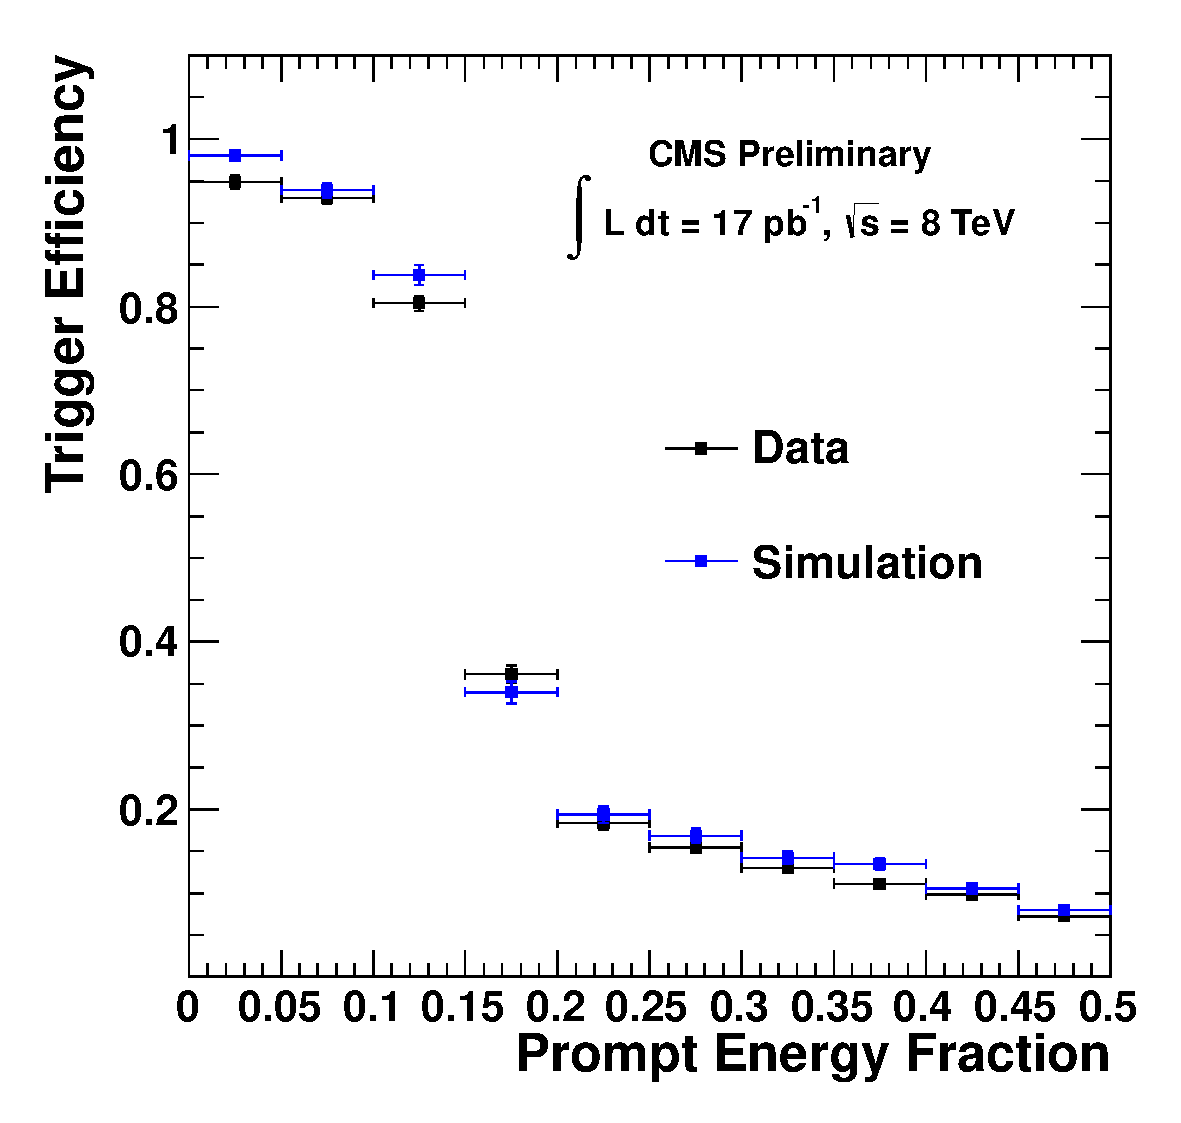
\includegraphics[width=0.49\textwidth]{plots/trigger/effHT300_PF_PromptEnergyFrac.pdf}
\caption{Single jet efficiency for jets with maximally 15\% prompt energy fraction as a function of offline prompt energy fraction. \label{fig:eff2PF}}
\end{figure}     

Systematic differences between data and simulation are again studied after applying the offline selection at 15\%.
 The efficiency as a function of $p_T$, $\eta$, $\phi$ is presented in Figure \ref{fig:eff2PFptetaphi}. 
The same procedure as in Section 
\ref{subsubsec:trig2Trks} is followed and the efficiency ratios are fitted with a zeroth order polynomial.
 No error inflation is needed as the statistical uncertainties on the individual ratio bins are larger
due to limited statistics.
 We assign a correction of 97\% and a conservative systematic uncertainty of 2\% for
each jet passing this filter from the average and the spread of the fit results for $p_T$, $\eta$, and $\phi$.
Similar performance of the filters in Sections \ref{subsubsec:trig2Trks} and \ref{subsubsec:trig2PF} 
is expected since both filters use properties of the similar sets of tracks.

\begin{figure}[!h]
\centering
 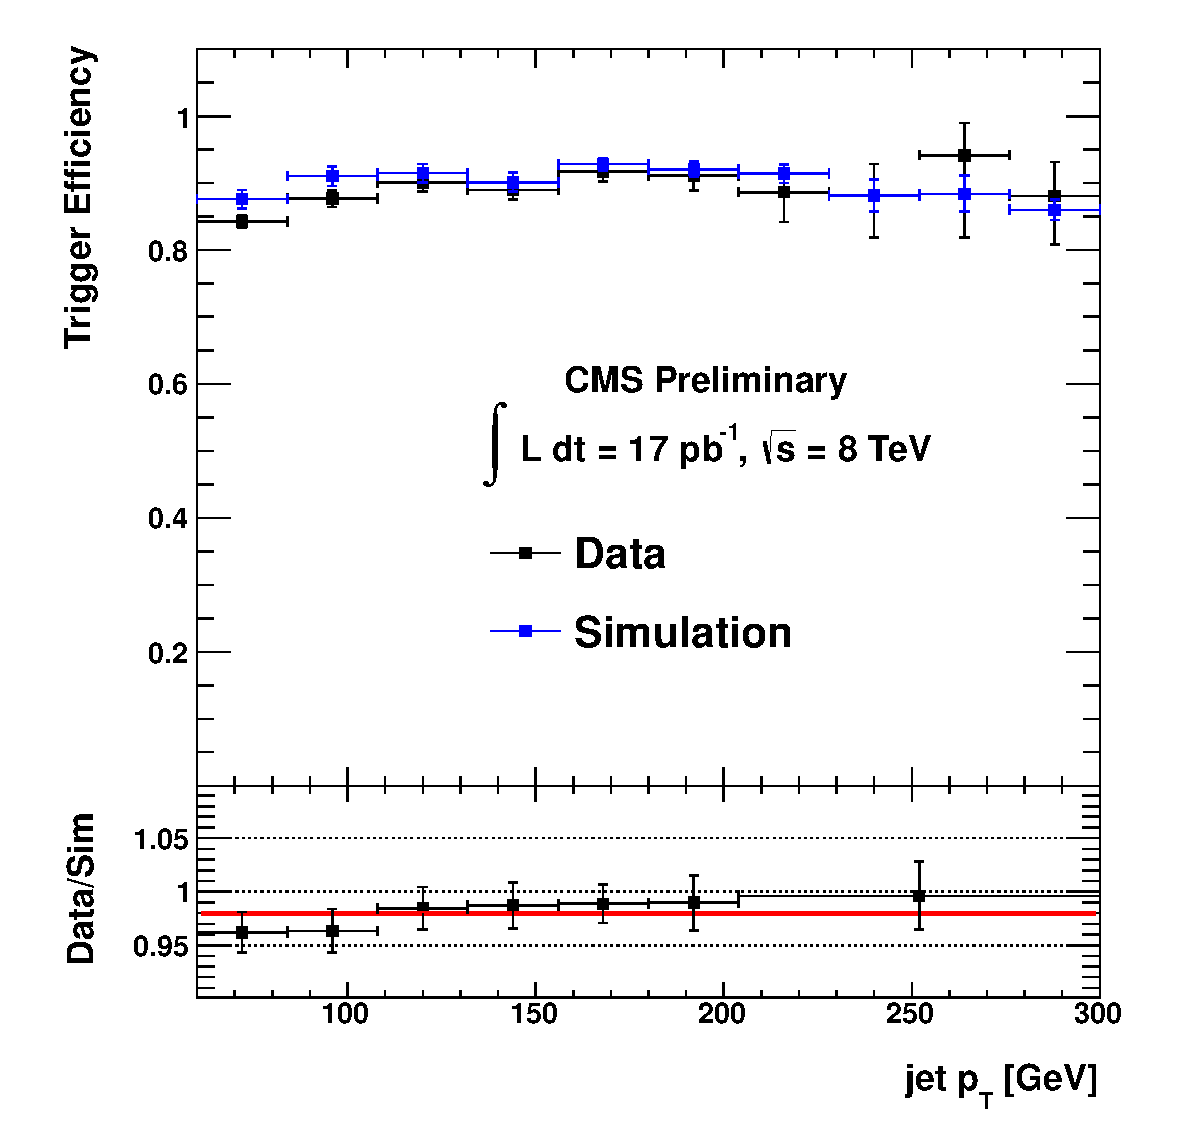
\includegraphics[width=0.32\textwidth]{plots/trigger/effHT300_PF_Pt.pdf}
 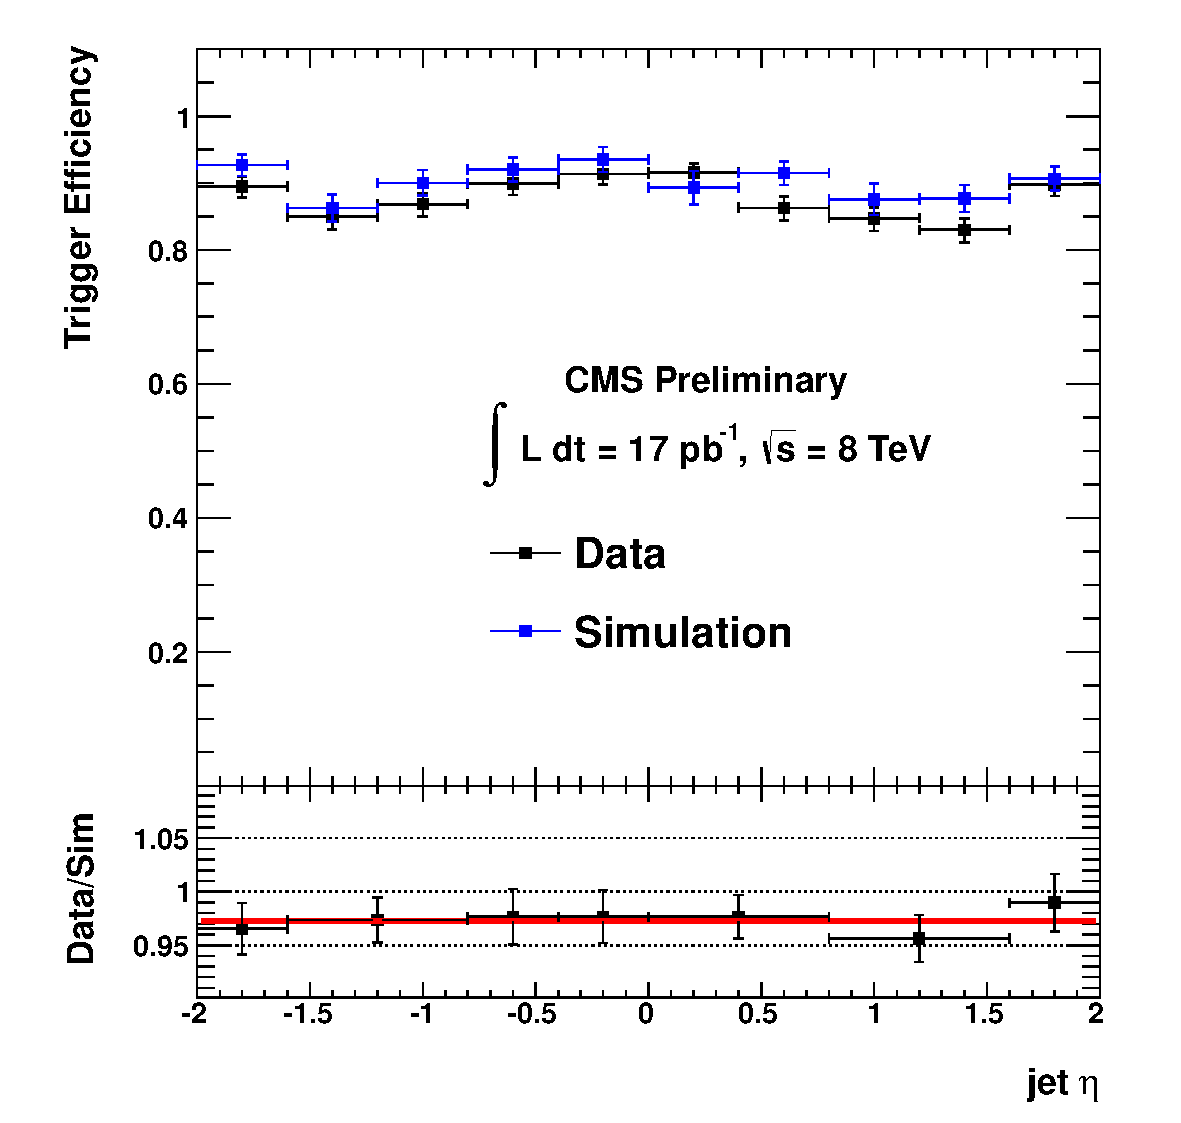
\includegraphics[width=0.32\textwidth]{plots/trigger/effHT300_PF_Eta.pdf}
 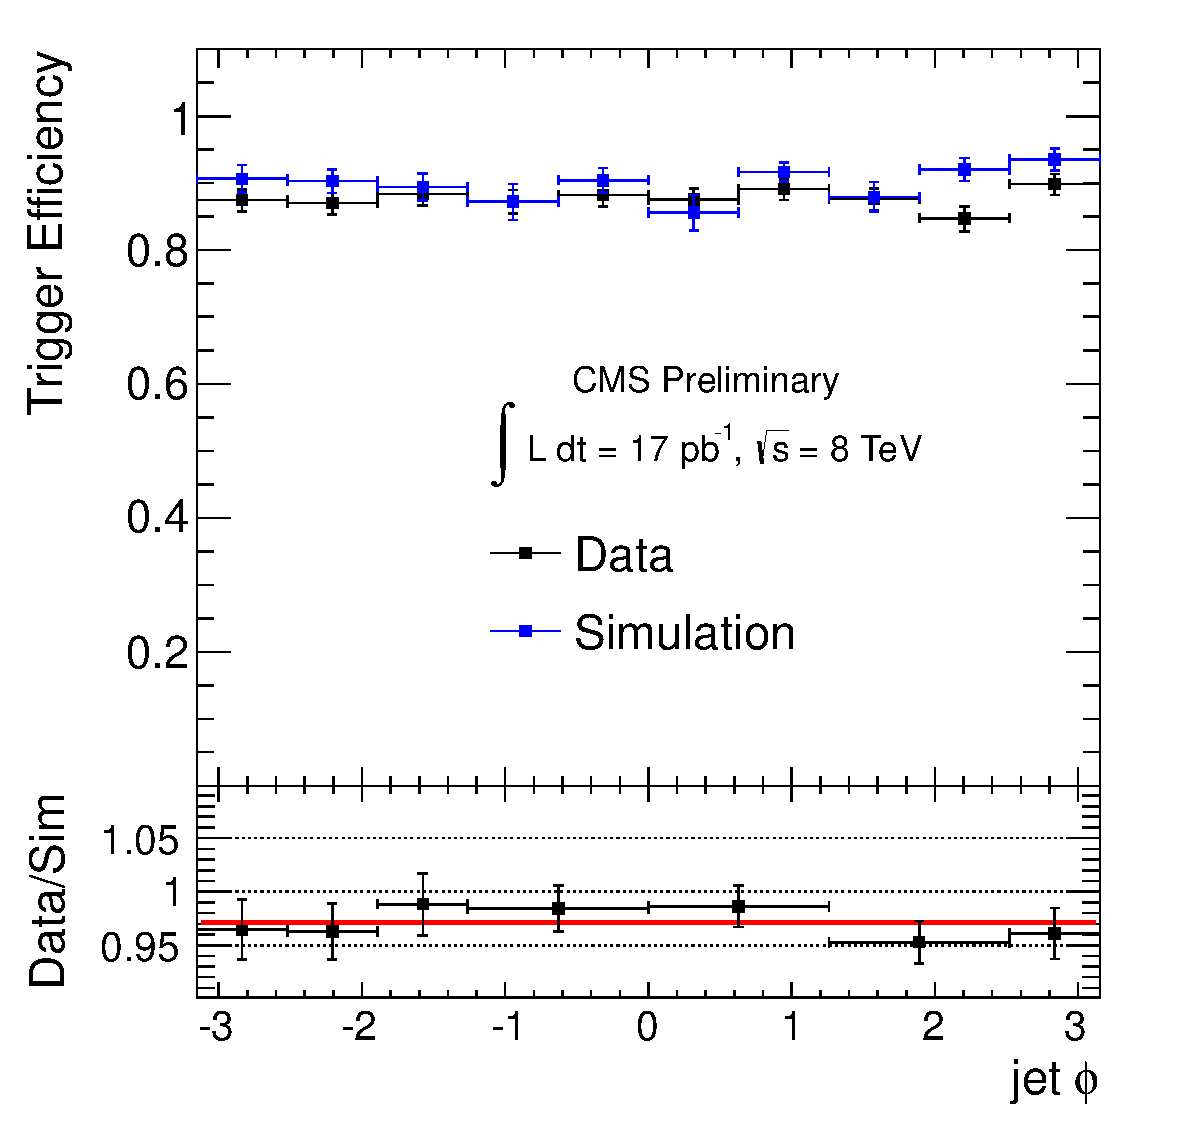
\includegraphics[width=0.32\textwidth]{plots/trigger/effHT300_PF_Phi.pdf}
\caption{Single jet efficiency as a function of jet $p_T$, $\eta$ and $\phi$ for jets with maximally 15\% prompt energy fraction. \label{fig:eff2PFptetaphi}}
\end{figure}

\subsubsection{Overall trigger efficiency}

Each of the trigger filters have been analyzed individually by determining performance differences 
between data and simulation. Observable discrepancies are accounted for as corrections in Sections
 \ref{subsubsec:trig2Trks} and \ref{subsubsec:trig2PF} and the uncertainties on the corrections are treated as 
systematic uncertainties. The trigger used in the analysis, HLT\_HT300\_DoubleDisplacedPFJet60, requires
 at least two jets passing the filters from Sections \ref{subsubsec:trig2Trks} and \ref{subsubsec:trig2PF}, 
hence corrections need to be applied twice, while systematic uncertainties added as fully correlated. 
Additionally, systematic uncertainties related to filters from Sections 
\ref{subsubsec:trig2Trks} and \ref{subsubsec:trig2PF} are both related to reconstruction of prompt tracks, therefore
 we adopt a conservative approach and add them as correlated also. The systematic uncertainty assigned to 
the filter from Section 
\ref{subsubsec:trigHT} is related to the jets transverse energy, hence it can be treated as uncorrelated. 
The total correction applied to the trigger efficiencies determined from simulation is thus 0.89 with a total
relative systematic uncertainty of 6\%. 

\subsection{Signal efficiency systematic}

Table \ref{tab:signalsystematics} summarizes the sources of systematic uncertainties on the signal efficiency
which add up to the total uncertainty between 8-10\% depending on the signal model.

\begin{table}[htbp]
\centering
 \begin{tabular}{r|l}
  Source & Uncertainty \\
  \hline
  Trigger efficiency & 6\% \\
  Tracking efficiency & 4\% \\
  Jet energy scale & 3-5\%(*) \\
  Jet momentum bias & 1-5\% \\ 
  %NLO effects & 3-20\%(*) \\ 
  Pile-up modelling & 2\% \\
%  Parton distribution functions & 1\% \\
  \hline
 Total & 8-10\% \\
 \end{tabular}
\caption{Summary of signal efficiency systematic uncertainties. *Applies only to samples with
 \Higgs mass of 200 and 400 \GeV.
\label{tab:signalsystematics}}
\end{table} 
